% Exemplo de monografia do IFG com texto em portugues formatado com LaTeX
\documentclass[
	% -- opções da classe memoir --
	oneside,
    %twoside,			% para impressão em verso e anverso. Oposto a oneside
	a4paper,			% tamanho do papel.
	% -- opções da classe abntex2 --
	chapter=TITLE,		% títulos de capítulos convertidos em letras maiúsculas
	%section=TITLE,		% títulos de seções convertidos em letras maiúsculas
	%subsection=TITLE,	% títulos de subseções convertidos em letras maiúsculas
	%subsubsection=TITLE,% títulos de subsubseções convertidos em letras maiúsculas
	% -- opções do pacote babel --
	english,			% idioma adicional para hifenização
	%french,				% idioma adicional para hifenização
	%spanish,			% idioma adicional para hifenização
	brazil				% o último idioma é o principal do documento
	]{cls/ifg}

% ---
% Pacotes básicos
% ---

\usepackage[T1]{fontenc}		% Selecao de codigos de fonte.
\usepackage[utf8]{inputenc}		% Codificacao do documento (conversão automática dos acentos)
% --- 		
% ---
% Pacotes adicionais, usados apenas no âmbito do Modelo Canônico do abnteX2
% ---
\usepackage{lipsum}				% para geração de dummy text
\usepackage{graphicx,multirow}
\usepackage[table,xcdraw]{xcolor}
\usepackage{setspace}
% ---

% ---
% Pacotes de citações
% ---
\usepackage[alf,abnt-and-type=e, abnt-year-extra-label=yes,abnt-url-package=html, abnt-repeated-author-omit = yes]{abntex2cite} %              	% Citações padrão ABNT
\usepackage{lastpage}
\usepackage{indentfirst}

% gantt gráfico para cronograma
\usepackage{pgfgantt}
% ---
% Informações de dados para CAPA e FOLHA DE ROSTO
% ---
%------------------------------------------ AUTOR, TÍTULO E DATA DE DEFESA %
\autor{Patrick Cavalcante Moraes}
\referenciaautor{MORAES, Patrick Cavalcante}

\titulo{SAD - SISTEMA PARA AVALIAÇÃO DE DESEMPENHO DOCENTE DO INSTITUTO FEDERAL DE GOIÁS}

\local{Luziânia}
\data{2021}
\orientador{Wendell Bento Geraldes}
\instituicao{Instituto Federal de Educação, Ciência e Tecnologia de Goiás}
\curso{Bacharelado em Sistemas de Informação}
\tipotrabalho{Trabalho de Conclusão de Curso} %Trabalho de Conclusão de Curso
% O preambulo deve conter o tipo do trabalho, o objetivo,
% o nome da instituição e a área de concentração

%\preambulo{Trabalho de Conclusão de Curso apresentado à Co-ordenação do Curso de Tecnologia em Análise e Desenvolvimento de Sistemas do Instituto Federalde Educação, Ciência e Tecnologia de Goiás - Câm-pus Luziânia, como requisito parcial para obtençãodo título de Tecnólogo em Tecnologia em Análisee Desenvolvimento de Sistemas.}

\preambulo{Projeto apresentado ao Curso de Bacharelado em Sistemas de Informação como um dos pré-requisitos de matrícula na Disciplina de Trabalho de Conclusão de Curso.}
% ---

% alterando o aspecto da cor azul
\definecolor{blue}{RGB}{41,5,195}
% informações do PDF
% ---
% Configurações de aparência do PDF final


\makeatletter
\hypersetup{
     	%pagebackref=true,
		pdftitle={\@title},
		pdfauthor={\@author},
    	pdfsubject={\imprimirpreambulo},
	    pdfcreator={\@author},
		pdfkeywords={revisão sistemática}{teclado virtual}{teclados assistivos}{otimização de teclados}{trabalho acadêmico},
		colorlinks=true,       		% false: boxed links; true: colored links
    	linkcolor=blue,          	% color of internal links
    	citecolor=blue,        		% color of links to bibliography
    	filecolor=magenta,      	% color of file links
		urlcolor=blue,
		bookmarksdepth=4
}
\makeatother
% ---

% ---
% Espaçamentos entre linhas e parágrafos
% ---

% O tamanho do parágrafo é dado por:
\setlength{\parindent}{1.3cm}

% Controle do espaçamento entre um parágrafo e outro:
\setlength{\parskip}{0.2cm}  % tente também \onelineskip

% ---
% compila o indice
% ---
\makeindex
% ---

% ----
% Início do documento
% ----
\begin{document}

% Seleciona o idioma do documento (conforme pacotes do babel)
%\selectlanguage{english}
\selectlanguage{brazil}

% Retira espaço extra obsoleto entre as frases.
\frenchspacing

% ----------------------------------------------------------
% ELEMENTOS PRÉ-TEXTUAIS
% ----------------------------------------------------------
% \pretextual

% ---
% Capa
% ---
\imprimircapa
% ---

% ---
% Folha de rosto
% (o * indica que haverá a ficha bibliográfica)
% ---
\imprimirfolhaderosto*
% ---

% ---
%Inserir a ficha bibliografica
% ---
%% Isto é um exemplo de Ficha Catalográfica, ou ``Dados internacionais de
% catalogação-na-publicação''. Você pode utilizar este modelo como referência.
% Porém, provavelmente a biblioteca da sua universidade lhe fornecerá um PDF
% com a ficha catalográfica definitiva após a defesa do trabalho. Quando estiver
% com o documento, salve-o como PDF no diretório do seu projeto e substitua todo
% o conteúdo de implementação deste arquivo pelo comando abaixo:
%
% \begin{fichacatalografica}
%     \includepdf{fig_ficha_catalografica.pdf}
% \end{fichacatalografica}

\begin{fichacatalografica}
	\sffamily
	\vspace*{\fill}					% Posição vertical
	\begin{center}					% Minipage Centralizado
	\fbox{\begin{minipage}[c][8cm]{13.5cm}		% Largura
	\small
	\imprimirautor
	%Sobrenome, Nome do autor
	
	\hspace{0.5cm} \imprimirtitulo  / \imprimirautor. --
	\imprimirlocal, \imprimirdata-
	
	\hspace{0.5cm} \pageref{LastPage} p. : il. (algumas color.) ; 30 cm.\\
	
	\hspace{0.5cm} \imprimirorientadorRotulo~\imprimirorientador\\
	
	\hspace{0.5cm}
	\parbox[t]{\textwidth}{\imprimirtipotrabalho~--~\imprimirinstituicao,
	\imprimirdata.}\\
	
	\hspace{0.5cm}
		1. Palavra-chave1.
		2. Palavra-chave2.
		2. Palavra-chave3.
		I. Orientador.
		II. Universidade xxx.
		III. Faculdade de xxx.
		IV. Título 			
	\end{minipage}}
	\end{center}
\end{fichacatalografica}
% ---


% ---
% Inserir errata
% ---
%\begin{errata}
Elemento opcional da \citeonline[4.2.1.2]{NBR14724:2011}. Exemplo:

\vspace{\onelineskip}

FERRIGNO, C. R. A. \textbf{Tratamento de neoplasias ósseas apendiculares com
reimplantação de enxerto ósseo autólogo autoclavado associado ao plasma
rico em plaquetas}: estudo crítico na cirurgia de preservação de membro em
cães. 2011. 128 f. Tese (Livre-Docência) - Faculdade de Medicina Veterinária e
Zootecnia, Universidade de São Paulo, São Paulo, 2011.

\begin{table}[htb]
\center
\footnotesize
\begin{tabular}{|p{1.4cm}|p{1cm}|p{3cm}|p{3cm}|}
  \hline
   \textbf{Folha} & \textbf{Linha}  & \textbf{Onde se lê}  & \textbf{Leia-se}  \\
    \hline
    1 & 10 & auto-conclavo & autoconclavo\\
   \hline
\end{tabular}
\end{table}

\end{errata}
% ---

% ---
% Inserir folha de aprovação
% ---

%% Isto é um exemplo de Folha de aprovação, elemento obrigatório da NBR
% 14724/2011 (seção 4.2.1.3). Você pode utilizar este modelo até a aprovação
% do trabalho. Após isso, substitua todo o conteúdo deste arquivo por uma
% imagem da página assinada pela banca com o comando abaixo:
%
% \includepdf{folhadeaprovacao_final.pdf}
%
\begin{folhadeaprovacao}

  \begin{center}
    {\ABNTEXchapterfont\large\imprimirautor}

    \vspace*{\fill}\vspace*{\fill}
    \begin{center}
      \ABNTEXchapterfont\bfseries\Large\imprimirtitulo
    \end{center}
    \vspace*{\fill}

    \hspace{.45\textwidth}
    \begin{minipage}{.5\textwidth}
        \imprimirpreambulo
    \end{minipage}%
    \vspace*{\fill}
   \end{center}

   %Trabalho aprovado. \imprimirlocal, \imprimirdata:

   \assinatura{\textbf{\imprimirorientador} \\ Orientador\\ \imprimirinstituicao}
   \assinatura{\textbf{Professor 1} \\ Membro da Banca \\ \imprimirinstituicao}

   \assinatura{\textbf{Professor 2} \\ Membro da Banca \\ \imprimirinstituicao}
   %\assinatura{\textbf{Professor} \\ Convidado 3}
   %\assinatura{\textbf{Professor} \\ Convidado 4}

   \begin{center}
    \vspace*{0.5cm}
    {\large\imprimirlocal}
    \par
    {\large\imprimirdata}
    \vspace*{1cm}
  \end{center}

\end{folhadeaprovacao}
% --- 


% ---
% Dedicatória
% ---
%\begin{dedicatoria}
   \vspace*{\fill}
   \centering
   \noindent
   \textit{ \textless dedicatória\textgreater} \vspace*{\fill}
\end{dedicatoria}
% --- 


% ---
% Agradecimentos
% ---
%\begin{agradecimentos}
...
\end{agradecimentos}
% --- 


% ---
% Epígrafe
% ---
%\begin{epigrafe}
    \vspace*{\fill}
	\begin{flushright}
		\textit{"Problemas não são obstáculos, mas oportunidades ímpares de superação e evolução."\\
		(Maurício Rodrigues de Morais)}
	\end{flushright}
\end{epigrafe}
% --- 

% ---
% RESUMOS
% ---
\setlength{\absparsep}{18pt} % ajusta o espaçamento dos parágrafos do resumo

% resumo em português
%\begin{resumo}

\imprimirreferenciaobra

\textless resumo do trabalho\textgreater


\textbf{Palavras-chave}: \textless palavrachaves separaradas por ;\textgreater.
\end{resumo} 


% resumo em inglês
%\begin{resumo}[Abstract]
 \begin{otherlanguage*}{english}

\textless resumo em inglês do trabalho\textgreater
   \vspace{\onelineskip}

   \noindent
   \textbf{Keywords}:\textless palavrachaves separaradas por ;\textgreater.
 \end{otherlanguage*}
\end{resumo} 

% resumo em francês
%\begin{resumo}[Résumé]
 \begin{otherlanguage*}{french}
    Il s'agit d'un résumé en français.

   \textbf{Mots-clés}: latex. abntex. publication de textes.
 \end{otherlanguage*}
\end{resumo}


% resumo em espanhol
%\begin{resumo}[Resumen]
 \begin{otherlanguage*}{spanish}
   Este es el resumen en español.

   \textbf{Palabras clave}: latex. abntex. publicación de textos.
 \end{otherlanguage*}
\end{resumo}
% ---


% ---
% inserir lista de ilustrações
% ---
\pdfbookmark[0]{\listfigurename}{lof}
%\listoffigures*
\cleardoublepage
% ---

% ---
% inserir lista de tabelas
% ---
\pdfbookmark[0]{\listtablename}{lot}
%\listoftables*
\cleardoublepage
% ---


% ---
% inserir o sumario
% ---
\pdfbookmark[0]{\contentsname}{toc}
\tableofcontents*
\cleardoublepage
% ---



% ----------------------------------------------------------
% ELEMENTOS TEXTUAIS
% ----------------------------------------------------------
\textual

\chapter{Introdução} \label{introdução}

    A partir de 1990, começa a ser implantada no Brasil a avaliação de desempenho, apoiando nos pilares da burocracia, mas revestida de novos ideais, dentre: o foco na desburocratização, descentralização, a autonomia do gestor, a horizontalização e a maior participação da comunidade \cite{bresser}. Desse contexto, percebe-se que a racionalidade existente nas políticas educacionais do país tem a considerar o docente como agente essencial para o avanço da qualidade de ensino e demandar que o trabalho e a capacitação desses profissionais sejam avaliados. Surgindo a necessidade para elaboração de planos de carreira que potencializa a adoção da avaliação de desempenho docente.

    A Lei de Diretrizes e Bases da Educação (LDB), no art. 67, estabelece que, os sistemas de ensino promoverão a valorização dos profissionais da educação, assegurando-lhes, inclusive nos termos dos estatutos e dos planos de carreira do magistério \cite{lei9394}. A existência da avaliação de desempenho indica que: progressão funcional baseada na titulação ou habilitação, e na avaliação do desempenho \cite{lei9394}, são determinações que possuem a garantia para alcançar a progressão na carreira profissional, sendo submetido a avaliação e possuindo a titulação e habilitação necessárias.

    Considerando que a aprovação em avaliação de desempenho individual consta como requisito legal a ser observado e atendido para aquisição de direito à progressão funcional e promoção na carreira docente, conforme disciplinado pela Portaria MEC nº 554, de 20 de junho de 2013 \cite{reitoria}. A Comissão Permanente de Pessoal Docente (CPPD) do Instituto Federal de Goiás (IFG) (CPPD, Portaria nº 1792/2020), a fim de dar prosseguimento à rotina para promoção e progressão dos docentes do quadro permanente de pessoal do IFG efetuou a criação da Avaliação Docente. Com isso, neste trabalho descreve-se as diversas etapas do desenvolvimento de um Sistema de Avaliação Docente (SAD) para o Instituto Federal de Goiás.

    Foi verificado a necessidade da instituição em um sistema de avaliação de desempenho docente, onde observado que o modelo de avaliação aplicado pelos sistemas atuais, já não agrega resultados satisfatórios diante a necessidade atual do IFG. Sendo que o mesmo possui uma grande quantidade de dados que são mantidos e unificados manualmente. A utilização de um novo \textit{software} assumiria uma integridade no controle desses dados gerados. Ao desenvolver um SAD, é construído um sistema que contemple as recomendações da instituição, desde as ferramentas utilizadas, passando pela escolha das tecnologias de desenvolvimento, a preparação do sistema e a adequada da utilização dos resultados, até os métodos de implantação a ações de manutenção.

    Serão também abordadas as metodologias ágeis aplicadas na criação e entrega do produto, de forma que atendam o conjunto de práticas eficazes, que se destinam a produzir o sistema demonstrando uma qualidade em seus processos, em uma forma de gerenciar o projeto sendo adaptável às mudanças. Essa abordagem propôs melhorias na gestão e acelerar os desenvolvimento do projeto.

    Com base nisso, este projeto tem como objetivo apresentar a necessidade de um Sistema de Avaliação Docente (SAD) para o apoio das demandas de avaliação de desempenho docente da Comissão Permanente de Pessoal Docente em um sistema unificado e entregar uma melhoria importante para a organização, podendo assim facilitar o processo de progressão dos docentes da instituição.


\section{Problema e Hipótese}

    O problema escolhido foi: como auxiliar a equipe da CPPD na otimização do processo de avaliação de desempenho docente do Instituto Federal de Goiás?
    
    A inexistência de um sistema estruturado para avaliação de desempenho, somado à alta demanda, resulta em um grande trabalho manual dos professores responsáveis, pertencentes a CPPD, o projeto apoiará o processo de avaliação dos docentes, coordenadores de curso, coordenadores acadêmicos e/ou chefe de departamento.
    
    Nesse cenário, este trabalho visa atender a demanda da CPPD, e também mostrar que é possível desenvolver um sistema, que seja capaz de gerir as informações e organizar o processo. O sistema será responsável pela condução do processo de avaliação docente para a efetivação da progressão funcional dos mesmos.
    
    Surge então a necessidade da criação do \textit{software}, onde as avaliações serão armazenadas e servirão como histórico para esses colaboradores, e também serão utilizadas para melhoria e estruturação deste processo, tirando esses registros dos formulários \textit{on-line} que atualmente consistem em um sistema externo, não vinculado a instituição que contempla parte das avaliações e do sistema Q-Acadêmico responsável pela outra parcela das avaliações de desempenho docente. Neste trabalho será apresentado como o Instituto Federal de Goiás pode agregar com uma solução de pesquisa, que tem como proposta construir um Sistema de Avaliação Docente (SAD). Também serão observados seus benefícios como a redução de custos e o aumento da agilidade, da otimização em processos, da acessibilidade e disponibilidade e da segurança junto à CPPD.
    



\section{Justificativa}

    De acordo \citen{comissao} as Instituições de Ensino Superior (IES), de um modo geral, vem sendo alvo de inúmeras questões sobre sua atuação no contexto social, e a ausência de subsídios que apresentem respostas concretas às questões constantes tem provocado o descrédito quanto à responsabilidade social. Desta forma, surge no seu bojo uma latente questão: As Instituições de Ensino Superior vem atendendo à demanda e expectativas da sociedade brasileira, enquanto entidade responsável pela disseminação do conhecimento? 
    
    Conforme abordado por \citen{oliveira-castro} os sistemas de avaliação devem ser justos e imparciais, baseados em padrões de desempenho atingíveis, objetivos, claros e apoiados na realidade dos cargos ou postos de trabalho. Para tal, é necessário pesquisar os padrões desejáveis de desempenho junto aos ocupantes dos cargos e às respectivas chefias.
    
    Implantar um sistema de avaliação visa melhorar alguns pilares importantes para uma organização, podendo colocar como os principais: planejamento, produtividade, ética, desenvolvimento de carreira, excelência, melhoria no processo de trabalho, responsabilidade e comprometimento. Em geral, o sistema visa subsidiar informações a respeito do desempenho dos professores da Instituição, de modo a promover a melhoria do ensino. 

    Portanto, em suma, é importante destacar que as instituições estão cientes de seu valor no processo de desenvolvimento e crescimento institucional, considerando que os profissionais estão sendo exigidos cada vez mais se capacitar para o mercado. Logo a avaliação de desempenho apresenta-se como instrumento e ação capaz de sinalizar o desempenho e detectar alterações entre o planejado e o que está sendo executado, oferecendo, desta forma, subsídios para correção.

    Diante a esse cenário, o IFG apresenta aplicações ineficientes para a automatização dos processos de avaliações docentes. A CPPD possui uma necessidade de um \textit{software} que seja capaz de efetuar as avaliações dos docentes pertencentes a instituição, sendo apto de gerir as informações e consiga atender os requisitos conforme os parágrafos anteriores. O sistema visará entregar um processo integrado que seja preparado para criar e gerir as avaliações de desempenho para fins de progressão e promoção funcional.


\section{Objetivo} \label{Objetivo}
    Esta seção tem como finalidade apresentar os objetivos que precisam ser alcançados  para realização deste  projeto.

\subsection{Objetivo Geral} \label{Objetivo Geral}
    O objetivo geral deste projeto é melhorar o processo de avaliação de desempenho docente, contribuindo com a melhoria no processo de avaliação docente e posterior progressão funcional. Essa abordagem de avaliação irá auxiliar a descobrir os pontos fortes e fracos dos docentes, além do fato de que é uma forma importante para que os docentes entendam o processo de avaliação no trabalho. 


\subsection{Objetivos Específicos} \label{Objetivos Específicos}
    Com a finalidade de atingir o objetivo geral, este projeto tem os seguintes objetivos específicos:

    
\begin{itemize}
    \item {Fazer o levantamento de requisitos;}
    \item {Modelar os requisitos na forma de diagramas;}
    \item {Elaborar o projeto de software;}
    \item {Implementar o software;}
    \item {Apresentar o protótipo a CPPD;}
    \item {Efetuar os testes;}
    \item {Validar o protótipo;}
    \item {Avaliação do \textit{software} junto a CPPD;}

\end{itemize}





%\newpage
\chapter{Fundamentação Teórica}

  
\section{Avaliação Docente do Instituto Federal de Goiás}
    O Instituto Federal de Goiás dispõe da Comissão Permanente de Pessoal Docente, como responsável pelas avaliações de desempenho para fins de progressão e promoção funcional, formada por 9 membros pertencentes ao quadro de servidores do IFG (Atualizado em 19 de agosto de 2021). Atualmente a CPPD é responsável por cerca de 1300 docentes que são avaliados periodicamente \cite{cppd}.
    
    Conforme a legislação nacional lei nº 12.772 \citen{lei12772}, de 28 de dezembro de 2012 que dispõe sobre a estruturação do Plano de Carreiras e Cargos de Magistério Federal e lei nº 12.863 \citen{lei12863}, de 24 de setembro de 2013 que altera a lei 12.772, de 28 de dezembro de 2012, que dispõe sobre a estruturação do Plano de Carreiras e Cargos de Magistério Federal. O desenvolvimento na Carreira de Magistério Federal, ocorrerá mediante progressão funcional e promoção, na forma disposta nas leis, que estabelece diretrizes gerais para o processo de avaliação de desempenho para fins de progressão e promoção dos servidores pertencentes ao Plano de Carreiras e Cargos de Magistério Federal das Instituições Federais de Ensino vinculadas ao Ministério de Educação de que trata o Capítulo III da Lei 12.772, de 28 de dezembro de 2013.
    
    A organização do IFG contempla 14 campus, e atualmente possui como método a Ficha de Avaliação de Desempenho. A avaliação é feita em dois períodos ao ano, de acordo com a Resolução Consup IFG nº 040/2018 \citen{resolucao} e Regimento Geral do IFG, Art. 190-193,198-201 \citen{regimento}, avaliando a atuação dos Docente, atribuindo-lhe nota numa escala de 0(zero) à 10(dez). 
    
    Atualmente as avaliações docentes do Instituto Federal de Goiás são feitas em dois sistemas distintos e vinculados a uma planilha eletrônica pelos membros da CPPD, tornando-se um procedimento manual passível a falhas. Quando necessário por diversos motivos, a consulta de uma nota atribuída anteriormente, é solicitado para a CPPD a planilha que está armazenada a nota, este processo requer tempo, e um trabalho manual dos membros da comissão para que consigam disponibilizar essas notas. 
    
    São feitas três avaliações: a avaliação do aluno, a avaliação do chefe departamento ou coordenador de curso e a auto avaliação, gerando uma média aritmética com a nota do docente. É necessário a soma das três notas e a divisão pela soma das quantidades, um processo simples, porém que necessita de uma aplicação que consiga unificar as avaliações em um sistema moderno que possa modificar o processo para melhor.


    

\section{Gerenciamento de Requisitos de Software}

    Conforme \citen{requisitosSoftware} a gerência de requisitos, abrange as atividades que tem por objetivo designar os atributos para os requisitos do software, definir suas visualizações dos requisitos de forma que as priorizações e o rastreamentos dos requisitos possam ser realizados. O processo corresponde ao conjunto de atividades que auxilia a equipe do projeto a identificar, controlar e rastrear os requisitos, bem como as alterações nos requisitos em muitos momentos do projeto.

    A Figura 1 Atividade de Gerenciamento de Requisitos descrita por \citen{wiegers} visa abordar o processo de gerenciamento de requisitos passando por todas as fases que compõem o modelo de gestão. As fases são divididas em quatro, sendo elas: realização do controle de mudanças, controle das versões dos requisitos, realização do acompanhamento de todos os requisitos para visualizar os estados de cada um e o rastreamento dos requisitos.
    
    \begin{figure}[h]
    \centering
    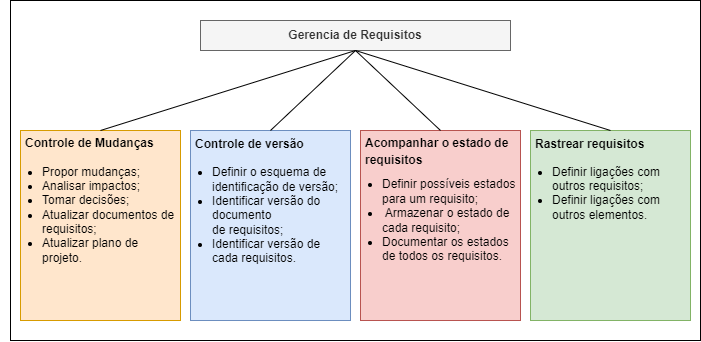
\includegraphics[width=1.0
    \textwidth]{./img/GerenciamentoRequisitos.png}
    \caption{Atividade de Gerenciamento de Requisitos \citen{wiegers}.}
    \label{fig:GerenciamentoRequisitos}
    \end{figure}
    
    O desenvolvimento de sistemas é fundamental que seja projetado para atender às necessidades do cliente. Para ajudar com a coleta das prioridades do usuário deve-se providenciar um levantamento de requisitos de \textit{software}. O levantamento de requisitos de software é um processo que serve para capturar as necessidades do cliente antes de projetar o desenvolvimento, evidenciando que os problemas solucionados pelo sistema serão problemas reais.
    
    Segundo \citen{centenaro} o diagrama de caso de uso documenta o que o sistema faz da perspectiva do usuário. Em outras palavras, descreve as principais funções do sistema e as interações dessas funções com os usuários. Neste diagrama, não será aprofundado nos detalhes técnicos, informando como o sistema funciona.
    
    \begin{figure}[h]
    \centering
    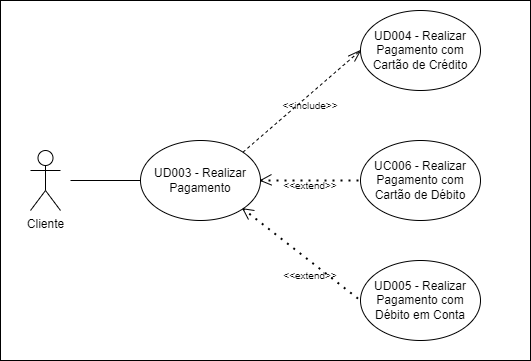
\includegraphics[width=0.78
    \textwidth]{./img/CasoUsoModelo.png}
    \caption{Modelo de Caso de Uso \citen{ventura}.}
    \label{fig:CasoUsoModelo}
    \end{figure}
    
    A abordagem utilizada no caso de uso acima visa descrever as interações entre o sistema com os usuários(atores), ou seja, como as funcionalidades se relacionam entre si e como serão utilizadas pelo usuário, durante o uso do sistema. Os três elementos citados no diagrama é o ator, casos de uso e os relacionamentos, sendo que o ator que fará a execução do caso de uso, já o caso de uso refere-se a interação que será tomada, portanto para que consiga efetuar o relacionamento existe os três principais relacionamentos que são: Inclusão (Include), Extensão (Extends) e Herança (Generalization).
    
    O relacionamentos possui a função de: \textit{Include}, quando o caso de uso A inclui o caso de uso B, significa que sempre que o caso de uso A for executado o caso de uso B também será executado. \textit{Extend}, quando o caso de uso B estende o caso de uso A, significa que quando o caso de uso A for executado o caso de uso B poderá ser executado também. E \textit{generalization} quando o caso de uso B generaliza o caso de uso C isso significa que, além de fazer tudo que está especificado em B, também executará tudo que está especificado no caso de uso C \cite{venturaP}.

    A Figura 2 exemplifica um diagrama de caso de uso com a função de realização de pagamento pelo cliente(ator). O caso de uso UD003 – Realizar Pagamento incluir a realização do pagamento com cartão de crédito pelo caso de uso UD004 – Realizar Pagamento com Cartão de Crédito e pode se estender com o pagamento com cartão de débito ou débito em conta pelos casos de uso UC006 – Realizar Pagamento com Cartão de Débito e UD005 – Realizar Pagamento com Débito em Conta.

    
\section{Metodologia Agil}

    Metodologia Ágil é um conjunto de práticas para entender as demandas de um projeto, agir e realizar tudo com eficiência. É uma ponte que tenta eliminar as lacunas no processo de desenvolvimento de software e entregar o produto final com mais rapidez e agilidade, sempre com qualidade \cite{jonatan}. Contudo a Metodologia ágil é uma forma de conduzir projetos que busca dar maior rapidez aos processos e à conclusão de tarefas.
        
        
\subsection{Scrum}

     Segundo \citen{scrum} o \textit{Scrum} é um método ágil para gestão de projetos. Sendo muito utilizado em equipes de desenvolvimento de software porque reúne um conjunto de boas práticas que facilitam o trabalho em equipes dessa natureza, como reuniões periódicas, lista de requisitos a serem atendidos, \textit{feedbacks} constantes sobre o produto, entre outros.
    
    O \textit{Scrum} é extremamente prescritivo, ou seja, para que um projeto dê certo dentro desse método é preciso seguir suas principais recomendações à risca, já que o Scrum define desde os papéis dentro da equipe de trabalho até a duração ideal das reuniões \cite{kanban}. No \textit{Scrum} exige que seja identificada uma lista de funcionalidades que precisam ser desenvolvidas para que o produto chegue ao objetivo esperado, o chamado \textit{Product Backlog} ou \textit{Backlog}. Essa lista é traduzida em \textit{Sprints}: ciclos de tempo onde pequenas partes do produto são planejadas, executadas e entregues, e é justamente aí que o \textit{kanban} pode entrar como um facilitador.

     Baseando-se na metodologia ágil, no \textit{framework Scrum}, onde as tarefas são reunidas em um  \textit{backlog}, e o projeto é dividido em blocos fixos de tempo com suas próprias tarefas e metas, ou seja, os \textit{sprints}, pode ser divididas as etapas de desenvolvimento do projeto. Outro ponto bastante utilizado da metodologia ágil, sendo suficiente apenas ter um \textit{backlog} com as entregas pendentes do projeto, uma forma simples, pois o foco será em antecipar o máximo possível o trabalho \cite{juliana}.
    
    Durante o desenvolvimento do produto, são definidas as etapas divididas em \textit{sprint}, conforme abordado por \citen{cronapp} “Um \textit{sprint backlog} é um tempo predeterminado que define o ciclo de desenvolvimento de um  \textit{software}”. Cada \textit{sprint} precisará ser validado, a partir da validação será iniciado um novo \textit{backlog} do sistema. 
    
    Também pode ser utilizado no desenvolvimento do sistema o \textit{Time Box} do \textit{Scrum} , na tradução literal significa “caixa de tempo”. Ou seja, é ter o tempo, para fazer um trabalho, limitado, executando da melhor forma que puder nessa janela de tempo. É uma técnica simples usada no desenvolvimento de software para rastrear o progresso e para, simplesmente, ter o trabalho feito e obter uma entrega contínua.
    
    
\subsection{Kanban}

    De acordo com \citen{digite} o \textit{Kanban} é um sistema de gestão visual para controle de tarefas e fluxos de trabalho através da utilização de colunas e cartões, facilitando a gestão de atividades. Sendo muito comum confundir o \textit{Kanban} com o \textit{Scrum}, ou achar que o \textit{Scrum} necessariamente precisa do \textit{Kanban} para funcionar.   
    
    
    O \textit{Kanban} é um sistema, ou seja, uma ferramenta para auxiliar no trabalho da equipe, como uma linguagem de programação, por exemplo. O sistema \textit{kanban} não é prescritivo ou impõe regras para que o trabalho seja feito corretamente, apenas possibilita que o time de trabalho execute suas tarefas com mais clareza e colaboração. E é por isso que, obviamente, o \textit{kanban} não funciona como um substituto para o \textit{Scrum}, no entanto, se utilizados juntos podem formar uma junção perfeita \cite{kanban}.
    
    No \textit{Kanban} pode incorporar as \textit{Sprints} e traduzir todo o trabalho que precisa ser executado em cartões, facilitando a gestão das tarefas para agilizar as entregas e garantir autonomia, que pode atribuir as próprias tarefas, princípios tão importantes para que o \textit{Scrum} funcione da melhor maneira. Já no que se refere a controlar as atividades, o quadro kanban se torna eficiente no controle acompanhando a produtividade com o esperado. Assim é aplicado as recomendações ágil e as práticas e técnicas que são suportadas, usufruindo as melhores abordagens para um cenário de um desenvolvedor.
    
    \begin{figure}[h]
    \centering
    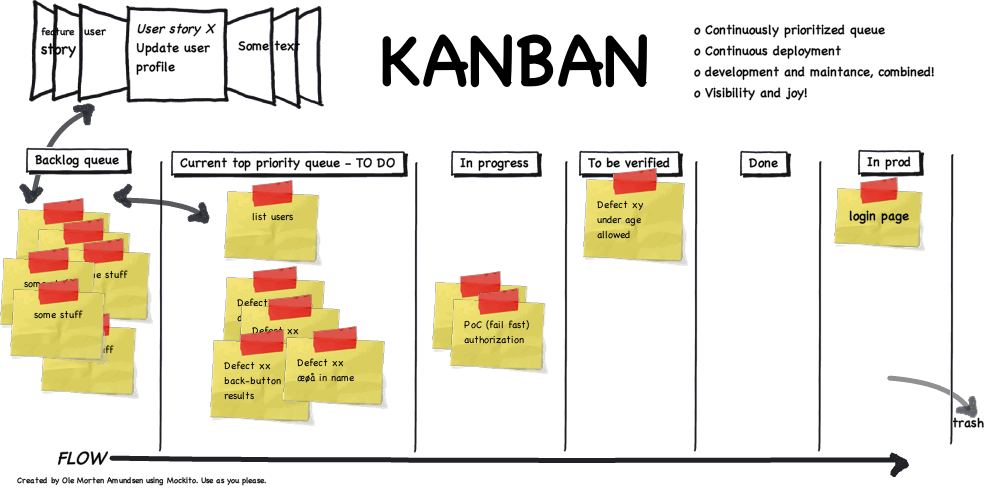
\includegraphics[width=1.0\textwidth]{./img/QuadroKanban.png}
    \caption{Modelo de Quadro Kanban \citen{ole}.}
    \label{fig:CasoUso}
    \end{figure}

    A Figura 3 demostra a estruturação de um quadro Kanban, evidenciando a estrutura dividida entre colunas com suas atividade. As colunas foram divididas respectivamente em: Fila de Pendências, Fila de Prioridade Máxima Atual - TO DO, Em Andamento, A Ser Verificado, Feito e Em Produção possuindo algumas atividade, como: página de login em produção, listar usuários na fila de prioridade máxima e falha rápida de autorização que está em andamento. Assim é um modelo que pode ser implementado de um quadro Kanban.

    Uma das ferramentas bastante utilizada na criação dos quadros \textit{Kanban} é o Trello. Segundo \citen{marc} o Trello é um “Quadro Kanban Online”, muito mais do que uma simples lista de tarefas ou \textit{task list}. Desta forma, pode-se criar diversos planos, cada um com seu respectivo quadro \textit{Kanban} e definir as etapas ou \textit{buckets} dos quadros. Além disso, pode convidar a equipe e criar, atribuir e acompanhar tarefas, movendo-as entre as colunas ou \textit{buckets}. Também pode utilizá-lo para planejar eventos, fornecer suporte, publicar conteúdos ou organizar um processo e criar quadros \textit{Kanban} usando tarefas de conteúdo avançado com recursos incluindo arquivos, listas de verificação e rótulos.

    \begin{figure}[h]
    \centering
    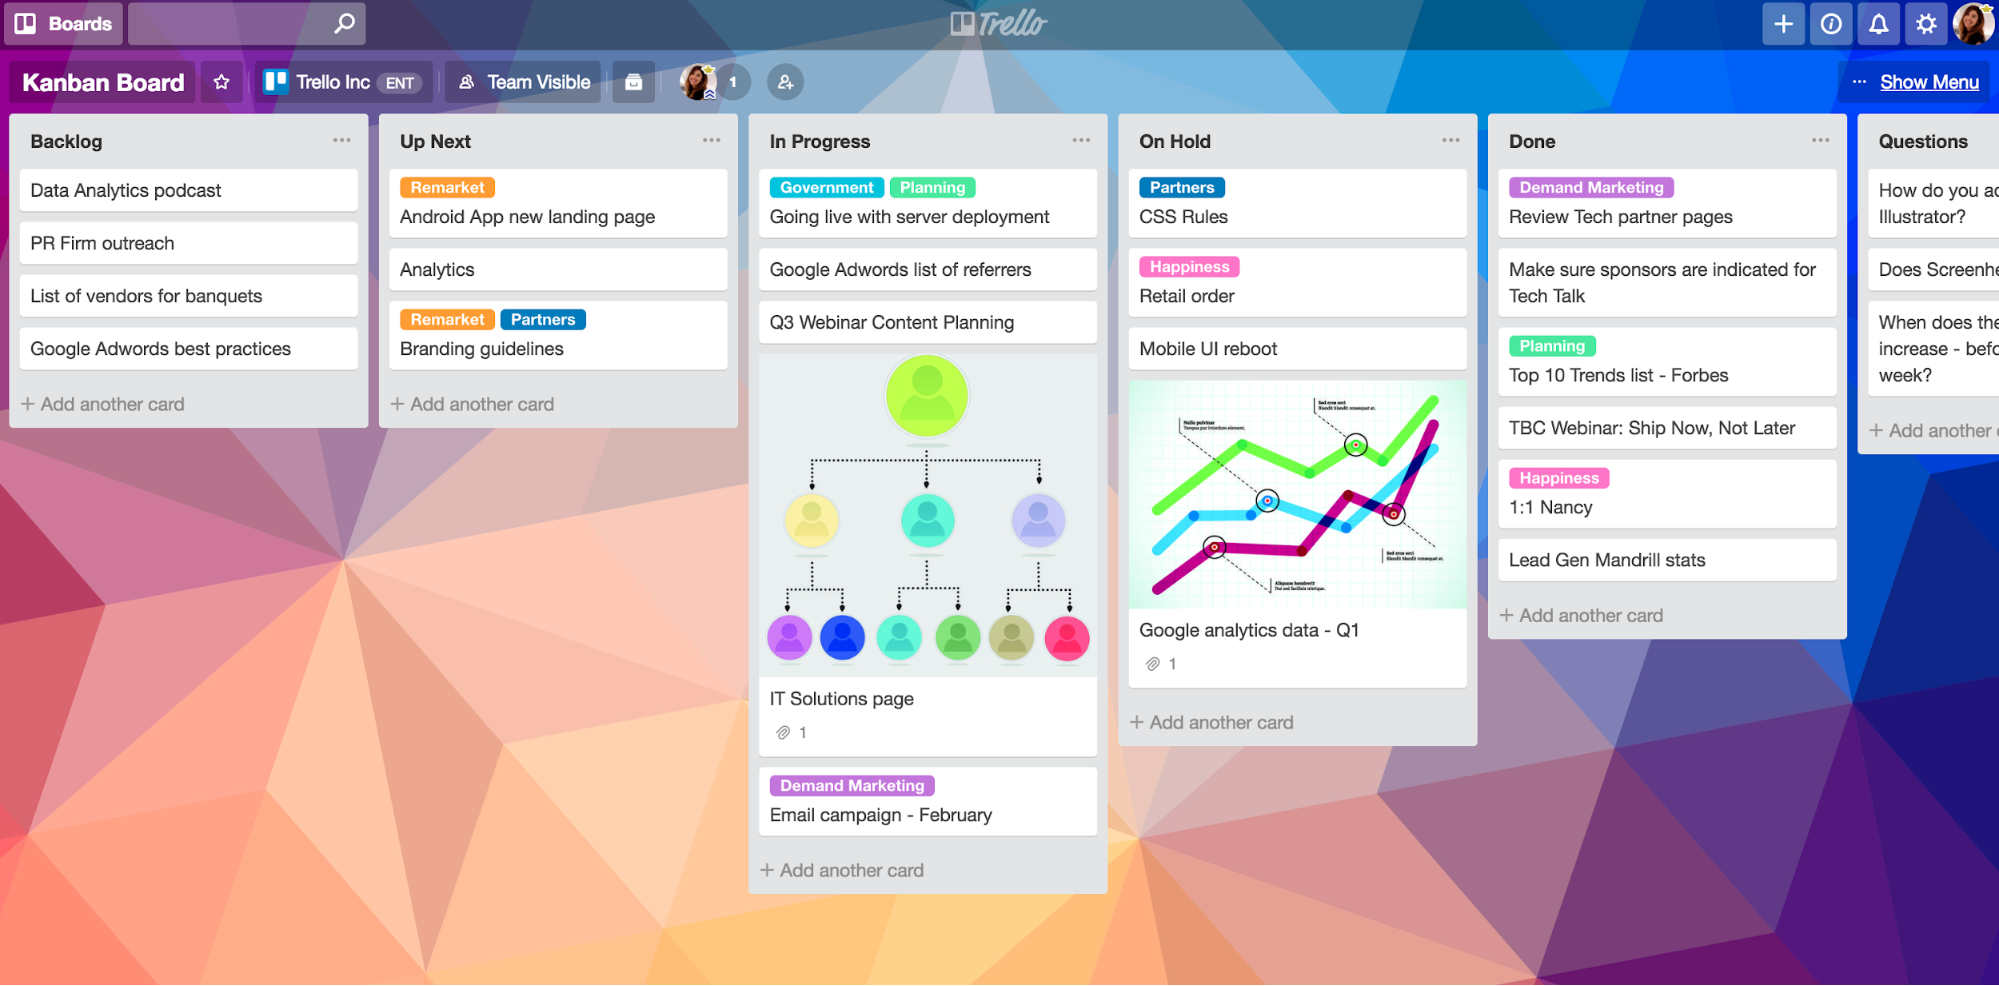
\includegraphics[width=1.0
    \textwidth]{./img/Trello.png}
    \caption{Trello - Gerenciamento de Tarefas \citen{rehkopf}.}
    \label{fig:Trello}
    \end{figure}

\section{API RESTful com Java 8 e Spring Boot}

    O mercado de desenvolvimento tem avançado e apresentado inúmeros recursos e padrões novos, que devem ser seguidos para atender a demanda de acessos e dados que precisam manipular nos dias de hoje. \textit{APIs RESTful} se tornaram peça chave para criação de aplicações robustas, seguindo padrões de micro serviços, além de trabalharem de modo \textit{standalone}, ou seja, sem que uma requisição dependa de outra para executar uma determinada operação \cite{souza}.

    É utilizado para a criação de diversas \textit{API RESTful} as tecnologias \textit{Java 8} e \textit{Spring Boot}, projetado para consumir informações da \textit{Web}. Segundo \citen{azevedo} essas aplicações têm por objetivo consumir informação por meio de interfaces que implementam uma série de rotinas e padrões que é chamada de API. O acrônimo API vem da expressão em inglês \textit{Application Programming Interface} (em português, Interface de Programação de Aplicações). Uma API é um conjunto de padrões e regras documentadas para que uma aplicação X possa utilizar funcionalidades de uma aplicação Y sem precisar conhecer os detalhes da implementação dessa aplicação X.

   Conforme \cite{vale} ao armazenar as senhas dos usuários na \textit{API Rest} a aplicação utiliza um modo seguro no banco de dados, utilizando o \textit{BCrypt} que permite encriptar irreversivelmente um certo valor, o que é ideal para armazenar informações com segurança em um banco de dados. O mais interessante é que, se chamado várias vezes, o \textit{BCrypt} criará diferentes valores de \textit{hash} para o mesmo valor, o que torna sua criptografia muito eficiente e segura, sendo a função \textit{hash} um algoritmo matemático para a criptografia, na qual ocorre uma transformação do dado (como um arquivo, senha ou informações) em um conjunto alfanumérico com comprimento fixo de caracteres.
   
   Ao desenvolver a \textit{API RESTful} pode-se implementar o \textit{BCrypt}, para o armazenamento correto das senhas no banco de dados, para que as senhas não fiquem claramente visíveis nas tabelas, se tornando um problema de segurança. O \textit{Spring Security} que é uma estrutura que se concentra em fornecer autenticação e autorização para aplicativos JAVA e que disponibiliza o mecanismos de codificação \textit{BCrypt}, também possui alguns outros mecanismos como \textit{MD5PasswordEncoder} e o \textit{ShaPasswordEncoder}, entretanto atualmente são considerados como obsoletos, por este motivo a melhor escolha é a implementação do \textit{BCrypt}.
   
    Desenvolvendo os componentes \textit{Spring} como serviços \textit{RESTful} da API, o \textit{Spring Rest} possui a anotação \textit{Controller} que uma vez adicionada a uma classe Java, aceitará um \textit{path} como parâmetro. Um objeto \textit{path} contém o nome do arquivo e a lista de diretórios usados para construir o caminho e é usado para examinar, localizar e manipular arquivos e também tornará esse componente disponível para acesso HTTP para o \textit{path} adicionado. Com os \textit{controllers}, é possível gerenciar os verbos HTTP (GET, POST, PUT, DELETE,...) para cada método da classe, permitindo criar todos os acessos RESTful para a API. 
        
    Conforme \citen{azevedo} o protocolo HTTP tem sido usado desde 1990 e a versão atual do protocolo é o HTTP/3. O protocolo define oito métodos que determinam ações a serem efetuadas no momento da requisição de algum recurso ao servidor. Desses oito, os 4 mais utilizados são:
    
    GET: método utilizado para ler e recuperar dados. Requisita uma representação do recurso especificado e retorna essa representação.
    
    POST: método utilizado para criar um novo recurso. Envia dados ao servidor. O tipo do corpo da solicitação é indicado pelo cabeçalho \textit{Content-Type}.
    
    PUT: cria um novo recurso ou substitui uma representação do recurso de destino com os novos dados. A diferença entre PUT e POST é que PUT é idempotente: ao chamá-lo uma ou várias vezes sucessivamente o efeito é o mesmo, enquanto se chamar o POST repetidamente pode ter efeitos adicionais. Por exemplo, se é criado um produto com POST, se a URL definida na API for chamada 20 vezes, 20 produtos serão criados e cada um deles terá um ID diferente. Já com o PUT, se você executar a URL definida na API 20 vezes, o resultado tem que ser o mesmo: o mesmo produto atualizado 20 vezes.
    
    DELETE: exclui o recurso.
    
    Para expor uma API com o Spring Boot, deve-se adicionar a dependência do \textit{Spring Boot Web}, para isso é adicionado ao arquivo pom.xml a tag <dependency>, com o endereço do framework e o artefato id conforme evidenciado na Figura 5.    

    \begin{figure}[h]
    \centering
    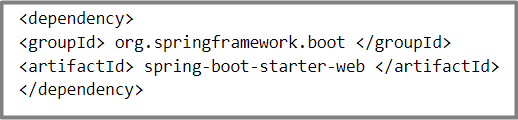
\includegraphics[width=0.75\textwidth]{./img/Dependência.png}
    \caption{Dependência Adicionadas.}
    \label{fig:Dependência}
    \end{figure}
    
    Após salvar o arquivo para instalar as dependências, que incluem o \textit{Tomcat, Jackson,} entre outras. Depois, é criado uma classe Java com o seguinte código:
    
    \begin{figure}[h]
    \centering
    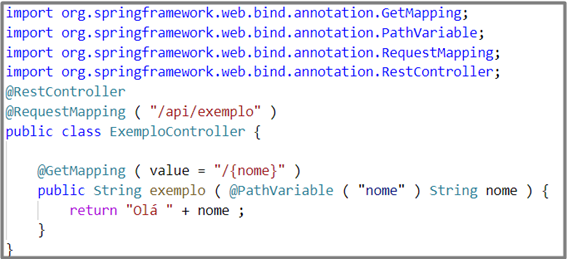
\includegraphics[width=0.85\textwidth]{./img/Classe.png}
    \caption{Criação da Classe.}
    \label{fig:Classe}
    \end{figure}
    
    No código acima, \textit{@RestControlle0r} é o responsável por criar a \textit{API Rest}, seguido do \textit{@RequestMapping}, que indicará o path do serviço. Após isso, basta mapear os métodos dos \textit{controllers} com a anotação \textit{@GetMapping}, seguido de um valor opcional como parâmetro. A \textit{@GetMapping} se refere a requisições HTTP GET, para outras como POST, PUT e DELETE, basta mudar a anotação para o formato desejado, como: \textit{@PostMapping, @PutMapping e @DeleteMapping,} respectivamente.

    Como demonstrado por \citen{souza} a \textit{@PathVariable} serve para obter um valor passado na URL nos serviços \textit{RESTful}, tanto os dados quanto as funcionalidades são considerados recursos e ficam acessíveis através da utilização de URIs. Essas URLs normalmente são endereços na web que identificam tanto o servidor no qual a aplicação está hospedada quanto a própria aplicação e qual dos recursos oferecidos pela mesma está sendo solicitado. Seguindo o mapeamento do exemplo abaixo, pode ser executada a aplicação e acessado com a seguinte URL para testar o controller.
    
    \begin{figure}[h]
    \centering
    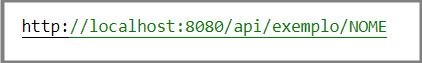
\includegraphics[width=0.45\textwidth]{./img/Endereço.png}
    \caption{URL de Acesso.}
    \label{fig:Endereço}
    \end{figure}
    
    
    Documentar uma aplicação é um ponto essencial de qualquer projeto, muitas vezes negligenciado. A partir da necessidade de documentar a \textit{API RESTful}, o recurso utilizado é o \textit{framework} Swagger, que é composto por diversas ferramentas que, independente da linguagem, auxilia a descrição, consumo e visualização dos serviços da API.

     Com o Swagger UI, a partir da especificação da API, pode-se criar documentações elegantes e acessíveis ao usuário, permitindo assim uma compreensão maior da API, pois além de poder ver os endpoints e modelos das entidades com seus atributos e respectivos tipos, o módulo de UI possibilita que os usuários da API interajam intuitivamente com a API usando uma sandbox. A sandbox é uma plataforma de testes onde as aplicações podem ser alteradas sem interferir no meio de produção. Nela, os desenvolvedores podem executar todas as operações de mudanças experimentais que vão garantir o bom funcionamento da solução, evitando danos que possam prejudicar o sistema \cite{diasW}.
     
    O \textit{Swagger} é a solução para documentar e criar ambientes para testes de uma \textit{API RESTful}, podendo facilmente integrado com o \textit{Spring Boot}, e de modo automático extrairá todas as informações da API do código-fonte. O modelo abaixo mostrar como as informações são documentadas no Swagger, mostrados os métodos implantados e os parâmetros necessários para as execuções.
    
    \begin{figure}[h]
    \centering
    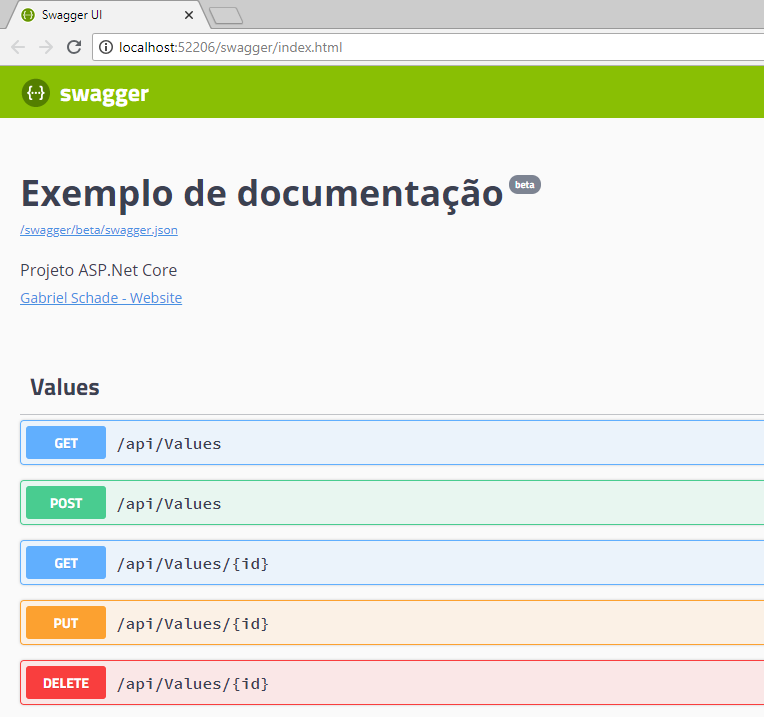
\includegraphics[width=0.80\textwidth]{./img/ExemploIUSwagger.png}
    \caption{Exemplo de IU do Swagger \citen{klaus}.}
    \label{fig:ExemploIUSwagger}
    \end{figure}

    Também pode fazer a utilização de um dos recursos disponíveis do \textit{Spring Boot} que desenvolve a criação de tabelas do banco de dados de modo automático. Com o \textit{Flyway} que é um \textit{framework} que permite o controle de versão e automação durante a criação do banco de dados, configurando a criação das tabelas, e os dados iniciais que devem estar na base de dados. O \textit{Flyway} também possui um utilitário de linha de comando que permite criar, atualizar e até mesmo limpar bancos de dados, tornando o gerenciamento de bancos de dados simples e intuitivo.

    Para a efetivação das requisições sem a necessidade de criar uma interface que execute a chamada, uma ferramenta bastante utilizada é o Postman. Conforme abordado por \citen{rodrigues} o Postman é uma aplicação que permite realizar requisições HTTP a partir de uma interface simples e intuitiva, facilitando o teste e depuração de serviços REST.


\section{Front-end com Angular 12}

    O \textit{framework} que está sendo mais utilizado atualmente para o desenvolvimento das interfaces web é o \textit{Angular 12}, plataforma de aplicativo \textit{web, front-end} e de código aberto, com a versão de produção mais recente, baseada na linguagem  de programação \textit{TypeScript}. Segundo \citen{angular} o angular é uma plataforma \textit{evergreen}, o que significa que se mantém atualizada com o ecossistema em evolução da \textit{web}. A remoção de suporte a navegadores legados é permitido concentrar os esforços em fornecer soluções modernas e melhor suporte aos desenvolvedores e usuários.
    
    Quando é construído uma interfaces com o Angula é criado componentes para cada uma das partes dessa interface, de forma que possa aproveitar em outras partes da aplicação sem repetição de código. Quando a prática de componentização e reaproveitamento chega ao extremo, pode-se utilizar bibliotecas de componentes prontas. Angular possui diversos recursos, e as bibliotecas fornecem elementos visuais e comportamentos padrão, que pode-se importar para a aplicação e utilizá-los, sem a necessidade de preocupar com templates \textit{HTML} e estilos \textit{CSS}. No universo \textit{Angular}, uma das bibliotecas mais utilizadas é o \textit{Angular Material} \cite{noleto}.

	Caso seja realmente necessário o Angular se comunicar com as bibliotecas JavaScript, um exemplo que pode ser utilizado é a integração com o \textit{jQuery} ao projeto Angular. O \textit{jQuery} está entre as mais utilizadas, se não a mais utilizada bibliotecas \textit{JavaScript}. A utilização de bibliotecas como facilitador no desenvolvimento de software, auxilia para que o tempo de desenvolvimento seja menor, com a reutilização de códigos existentes. No \textit{front-end} com Angula pode ser utilizadas bibliotecas de extensões para o \textit{JavaScript}, como:
    
\begin{itemize}

    \item \textit{jQuery}, é uma biblioteca livre que contém funções da linguagem de programação \textit{JavaScript} que interage com páginas em \textit{HTML}, desenvolvida para simplificar os \textit{scripts} executados e/ou interpretados no navegador de internet do usuário \cite{plinio};
    
    \item \textit{RxJS}, é uma biblioteca para programação reativa que possibilita o uso da programação para a linguagem de \textit{Java}, sendo uma biblioteca para compor programas assíncronos e baseados em eventos usando sequências \textit{Observables} \cite{rxjs};
    
    \item \textit{Moment.js}, é um pacote \textit{open source} que pode ser utilizado para validar, manipular e fazer o \textit{parse} de datas, definindo assim os valores de data baseados em \textit{string} no  \textit{JavaScript} \cite{moment}.

\end{itemize}

    Já \textit{Angular Material}, como abordado por \citen{material} os componentes do \textit{material design} para o \textit{Angular}, possui alta qualidade com componentes internacionalizados e acessíveis para todos, bem testado para garantir desempenho e confiabilidade, com \textit{APIs} simples, com comportamento consistente entre plataformas. Versátil, fornece ferramentas que ajudam os desenvolvedores a construir seus próprios componentes personalizados com padrões de interação comuns e customizáveis dentro dos limites da especificação do \textit{Material Design}.
    
        \begin{figure}[h]
        \centering
        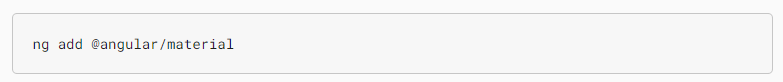
\includegraphics[width=0.80\textwidth]{./img/MaterialDesign.png}
        \caption{Exemplo de como adicionar a dependencia do Angular Material disponivel em \cite{material}.}
        \label{fig:MaterialDesign}
        \end{figure}

    De acordo com \citen{nodejs} projetos desenvolvidos que utilizam como padrão o \textit{Agular 12}, possui como requisito ao menos a versão 10 ou superior do \textit{NodeJS}, portanto é necessário instalar a versão \textit{NodeJS 10} para execução do projeto. Sendo o \textit{Node.js} um \textit{software} de código aberto, multiplataforma, baseado no interpretador V8 do \textit{Google} e que permite a execução de códigos \textit{JavaScript} fora de um navegador \textit{web}.
   

\section{Banco de Dados com PHPMyAdmin}
    Segundo \citen{dev}, um banco de dados é uma coleção de dados inter-relacionados, representando informações sobre um domínio específico, ou seja, sempre que for possível agrupar informações que se relacionam e tratam de um mesmo assunto, pode-se dizer que existe um banco de dados.
    
    Os bancos de dados desempenham um papel importante, senão fundamental, quando se trata de hospedagens. Como blogs, sites, lojas, aplicativos e diferentes tipos de sistemas online virtuais contam com esse recurso para armazenar todo tipo de informação. Qualquer aplicativo ou sistema baseado na web precisa de algum tipo de banco de dados. 
    
    \begin{figure}[h]
    \centering
    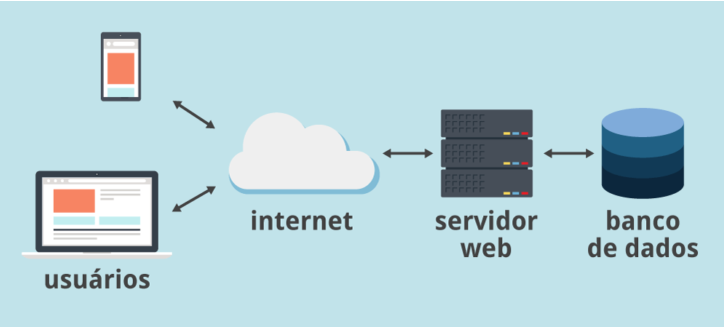
\includegraphics[width=0.55\textwidth]{./img/BancoDados.png}
    \caption{Componentes de um Sistema de Banco de Dados \citen{bordallo}.}
    \label{fig:BancoDados}
    \end{figure}

    A arquitetura mostrada na Figura 10 corresponde ao funcionamento de um sistema e como seus componente se interligam a um banco de dado. Os usuários acessam as suas interfaces do sistemas, que comunica com a internet. A internet nessa estrutura acessa o servidor web que armazena as informações em um banco de dados. Essa é uma arquitetura básica da comunicação de um sistema com um banco de dados.
    
    Conforme evidenciado por \citen{mer} pode-se desenvolver o diagrama de entidade relacional para facilitar o projeto lógico do banco de dados, permitindo a representação da estruturação lógica, sendo um dos modelos de dados com maior capacidade semântica e representa um problema como um conjunto de entidades e relacionamentos entre essas entidades.
    
    \begin{figure}[h]
    \centering
    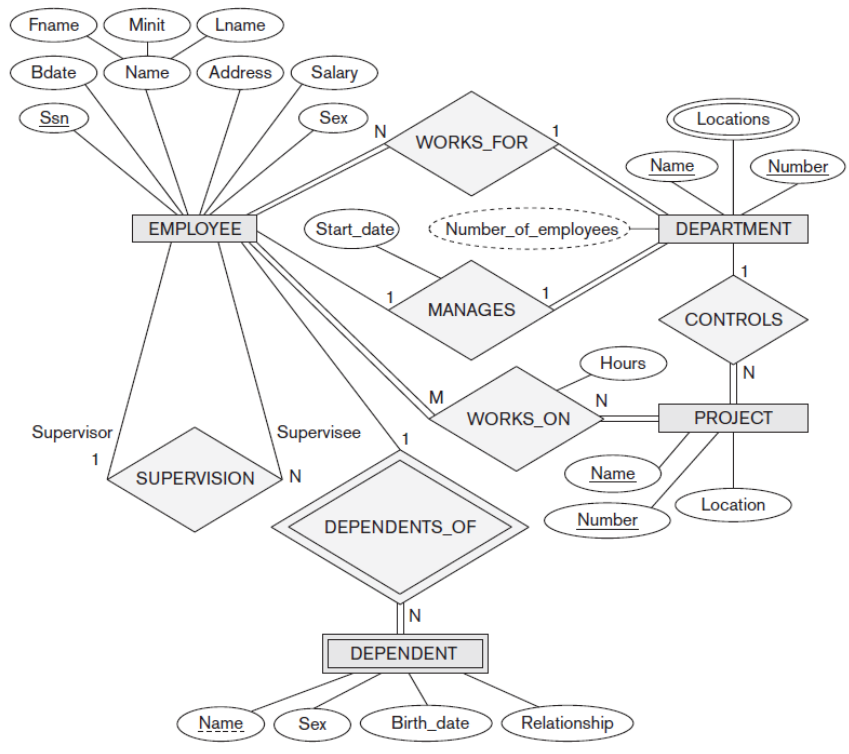
\includegraphics[width=0.75\textwidth]{./img/ExemploDiagramEntidadeRelacionamento.png}
    \caption{Exemplo de Diagrama de Entidade Relacionamento \citen{cavalcanti}.}
    \label{fig:ExemploDiagramEntidadeRelacionamento}
    \end{figure}

    Percebe-se a necessidade de armazenar e manipular dados e neste contexto é imprescindível que estes sejam armazenados de forma organizada e permitam um posterior acesso eficiente. Assim, torna-se necessário implementar o banco de dados. O Diagrama Entidade Relacionamento utiliza elementos gráficos para descrever o modelo de dados de um sistema com alto nível de abstração.

    Para \citen{macedo} o conceito básico de chave de um banco é que é uma ou mais colunas que distinguem uma linha das demais dentro de uma tabela, sendo esta chamada de chave primária (\textit{PK – Primary Key}) ou para relacionar com outra tabela, chamada de chave estrangeira (\textit{FK – Foreign Key}). Essas chaves é que determinam a unicidade de cada registro dentro de uma tabela.
   
 \subsection{PhpMyAdmin}
   O PhpMyAdmin é um administrador de bancos de dados em MySQL, proporcionando um trabalho de gestão e edição muito mais prático com aplicações. A ferramenta, de código aberto e uso livre, é voltada para desenvolvedores que trabalham desenvolvendo sites e ferramentas, e que precisam de uma interface mais simples. Seu principal papel é, justamente, tornar o trabalho mais simples \cite{souzaIvan}.
   
   A utilização do PhpMyAdmin é uma ferramenta destinada a lidar com a administração do Sistema de Gerenciamento de Banco de Dados (SGBD) MySQL pela Web, sendo o MySQL simplesmente um sistema que pode armazenar e gerenciar esses dados. Uma das principais características do PhpMyAdmin é a facilidade de se trabalhar com o SGBD MySQL, desenvolvida exclusivamente para o trabalho com o MySQL e também possui um foco na modelagem física.

   Umas das principais ferramentas utilizadas no gerenciamento do PhpMyAdmin em diferentes sistemas operacionais é o  XAMPP.  O XAMPP é um pacote com os principais servidores de código aberto do mercado, incluindo FTP, banco de dados MySQL e Apache com suporte às linguagens PHP e Perl segundo \citen{higa}.   
    
\subsection{Recursos Estimativos Para a Alta Performance}

    A abordagem da Figura 12 que pode-se utilizar no momento da implantação, visando o desempenho do banco de dados, é cria-se uma zona segura de processamento seguindo um padrão de escalar verticalmente, refere-se à quantidade que pode ser consumida sem atingir o limite de saturação. Neste cenário, a zona segura é considerada ao respeitar a quantidade de recursos estipulada, ou utilizando até 60\% de CPU.
   
    \begin{figure}[h]
    \centering
    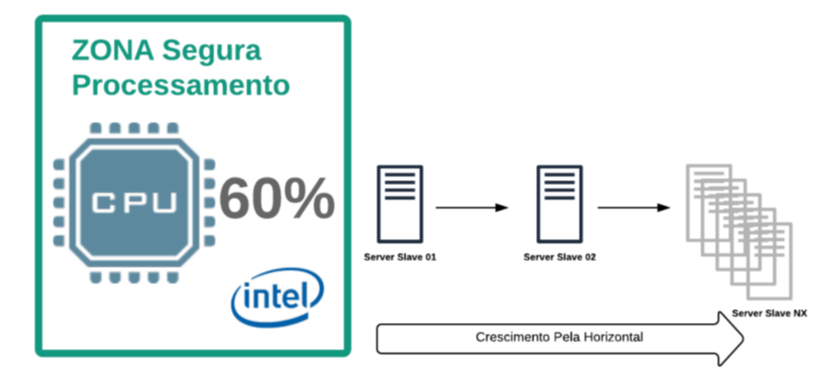
\includegraphics[width=0.90\textwidth]{./img/segProc.png}
    \caption{Modelo de Implementação do Banco de Dados \citen{totvs}.}
    \label{fig:segProc}
    \end{figure}

    Uma das recomendação que também pode ser seguida no momento da implantação do sistema, no \textit{hardware} físico indicado para uma melhor performance, o uso de volumes \textit{High Performance} (como \textit{SSD/Flash}), considerando a volumetria/conexões do ambiente.    
    
    
\section{Abordagens de Testes de Usabilidade e Desempenho do Sistema}

    Segundo \citen{patel} teste de usabilidade é um método de verificação de funcionalidades da interface de uma plataforma digital. É empregado em websites, aplicações e outras ferramentas, levando usuários reais à execução de determinadas tarefas. Após sua realização, é realizada uma análise de usabilidade e das principais dificuldades.
    
    Conforme abordado por \citen{desempenho} o teste de desempenho é uma classe de testes implementada e executada para caracterizar e avaliar as características relacionadas ao desempenho do destino do teste, como perfis de sincronização, fluxo de execução, tempos de resposta e confiabilidade e limites operacionais. 
    
    Portanto, ao realizar o teste enxergará a interface do ponto de vista de que a utilizará. Sendo efetuado o modelo de teste que visa a descoberta de problemas, esse modelo de teste quando aplicado, seu objetivo é identificar e corrigir eventuais problemas existentes na aplicação, observando quais são os obstáculos para a fluida utilização.

\subsection{Teste de integração com @SpringBootTest}

    O conceito de TDD (Desenvolvimento Guiado por Testes) define que antes de criar um código novo (classe), deve-se escrever um teste (classe de test case). Essa prática traz vários benefícios às equipes de desenvolvimento e inclusive estes testes serão usados como métrica em todo o tempo de vida do projeto. Na imagem abaixo um modelo de como funciona o processo de testes unitários dentro do projeto \cite{tdd}.
    
    \begin{figure}[h]
    \centering
    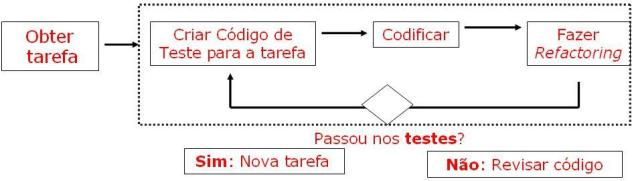
\includegraphics[width=0.95\textwidth]{./img/TDD.jpg}
    \caption{Processo de Testes Unitários \citen{tdd}.}
    \label{fig:TDD}
    \end{figure}
    
    No TDD para que possa obter um nova tarefa de desenvolvimento é necessário criar o código de teste para classe, codificar e efetuar a refatoração, caso a classe da tarefa passe no teste pode-se seguir para a criação de uma nova classe. Porém caso essa classe não passe no teste é necessário revisar o código e efetuar novamente o teste até que essa classe seja aprovada conforme mostrado na Figura 13.
    
    Uma abordagem que se utiliza no momento do desenvolvimento é o teste de integração, o \textit{Spring Boot} utilizado na criação da \textit{API RESTful} possui o mecanismo JUnit que após ser implementado possui testes unitários em Java. O JUnit é um framework que facilita o desenvolvimento e execução de testes unitários em código Java. Na imagem abaixo, apresenta um diagrama que mostra a forma como as classes de testes ficam organizadas em um projeto codificado em Java. 

    \begin{figure}[h]
    \centering
    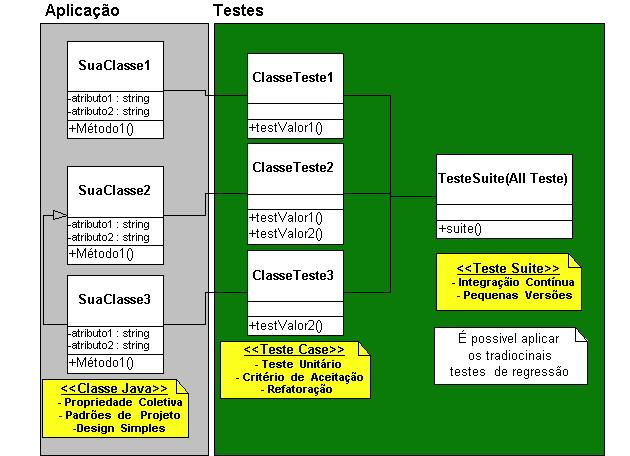
\includegraphics[width=0.85\textwidth]{./img/ClassesTeste.jpg}
    \caption{Organização das Classes de Testes \citen{tdd}.}
    \label{fig:ClassesTeste}
    \end{figure}

    Como o nome sugere, os testes de integração se concentram na integração de diferentes camadas do sistema. Idealmente, deve-se manter os testes de integração separados dos testes de unidade e não devem ser executados junto com os testes de unidade, porém pode-se fazer isso usando um perfil diferente para executar apenas os testes de integração. Algumas razões para realização nesse formato, podem ser que os testes de integração são demorados e pode precisar de um banco de dados real para serem executados. No entanto, também suporta a utilização do armazenamento de persistência H2 na memória.

    O H2 é um banco de dados em memória que permite todas as operações, permitindo assim testar as aplicações mesmo sem um banco de dados já definido, com um console acessível pelo browser dentro do contexto da aplicação.



 

\newpage
\chapter{Hipótese}
    A hipótese deste trabalho é apresentar como o Instituto Federal de Goiás pode agregar com uma solução de pesquisa, que tem como proposta construir um Sistema de Avaliação Docente, pois há uma inexistência de um sistema estruturado para avaliação de desempenhos, conforme descrito no capítulo 1.1(Problema). Também será observado seus benefícios como a redução de custos e o aumento da agilidade, da otimização em processos, da acessibilidade e disponibilidade e da segurança junto a CPPD.


\newpage
\chapter{Metodologia}
%    --Como atingir os objetivos especificos 
%    --Como vou fazer (Levantamento de requisito, Wendell.
%    Funcionais, não funcionais

    Nesta seção é apresentado como este projeto será desenvolvido para atingir o objetivo esperado. Sendo divido em quatro etapas:
    
    \begin{itemize}
        \item Na primeira etapa, será realizado uma pesquisa bibliográfica sobre o tema em livros, artigos, dissertações, teses e e-books. Para a busca deste material, serão utilizadas ferramentas online como Google Scholar, Jurn, CAPES, Bibliotecas digitais de universidades e a biblioteca da própria instituição.
    
        \item Na segunda etapa será levantado os requisitos definindo os requisitos funcionais e não funcionais. E a criação do diagrama de caso de uso, para concepção da visão geral do sistema. 
    
    	\item Na terceira etapa será criado o protótipo do sistema, aplicando os requisitos levantado na etapa anterior. Nesta etapa será desenvolvido a API REST e integrada com o framework Angular, aplicando no decorrer do desenvolvimento abordagens segundo a metodologias ágil Scrum.
    	
    	\item Na quarta e última etapa será efetuado uma comparação com os processos destacados anteriormente e a execução dos testes de aceitação do software juntamente com a CPPD. Criando possíveis novos pontos de função e melhorias para o sistema.

\end{itemize}



\chapter{Recursos Necessários}

Os recursos necessários para a criação do Sistema para Avaliação de Desempenho serão:
    
\begin{itemize}
    \item Computador com configuração mínima de, 3.0 GHz de processamento, 4Gb de RAM, 2Gb de espaço livre no HD;
    \item Papel Sulfite e cartuchos para impressão do trabalho;
    \item Internet para realizar as pesquisas;
    \item Sofware IDE de Desenvolvimento Intellij e SGBD MySQL Workbenck;
    \item A plataforma OverLeaf para o desenvolvimento do trabalho escrito.
\end{itemize}



\chapter{Cronograma}

    Esta seção apresenta o cronograma deste projeto, como será dividida as atividades dentro do tempo estimulado para a realização deste trabalho. 
    
\begin{itemize}
    \item \textbf{Atividade 1:} Fazer o levantamento de requisitos;
    \item \textbf{Atividade 2:} Modelar os requisitos na forma de diagramas;
    \item \textbf{Atividade 3:} Elaborar o projeto de software; 
    \item \textbf{Atividade 4:} Implementar o software;
    \item \textbf{Atividade 5:} Apresentar o protótipo a CPPD;
    \item \textbf{Atividade 6:} Validar o protótipo;
    \item \textbf{Atividade 7:} Efetuar os testes;
    \item \textbf{Atividade 8:} Escrita do projeto.
\end{itemize}

    Abaixo temos a tabela do cronograma a ser seguido:
    


% Tabela 1
%\begin{table}[h]
%    \centering
%% distancia entre a linha e o texto
% {\renewcommand\arraystretch{2}
% \begin{tabular}{ l l l l l l l l l l l l l l l l l l }
%  \cline{1-1}\cline{2-2}\cline{3-3}\cline{4-4}\cline{5-5}\cline{6-6}\cline{7-7}\cline{8-8}\cline{9-9}\cline{10-10}\cline{11-11}\cline{12-12}\cline{13-13}\cline{14-14}\cline{15-15}\cline{16-16}\cline{17%-17}\cline{18-18}  
%    \multicolumn{18}{|p{8.000cm}|}{\textbf{Cronograma} \centering }
%  \\  
%  \cline{1-1}\cline{2-2}\cline{3-3}\cline{4-4}\cline{5-5}\cline{6-6}\cline{7-7}\cline{8-8}\cline{9-9}\cline{10-10}\cline{11-11}\cline{12-12}\cline{13-13}\cline{14-14}\cline{15-15}\cline{16-16}\cline{17-17}\cline{18-18}  
%    \multicolumn{1}{|p{1.590cm}|}{\textbf{Atividade} \centering } &
%    \multicolumn{4}{p{1.000cm}|}{\textbf{Abril} \centering } &
%    \multicolumn{5}{p{1.000cm}|}{\textbf{Maio} \centering } &
%    \multicolumn{4}{p{1.000cm}|}{\textbf{Junho} \centering } &
%    \multicolumn{4}{p{1.000cm}|}{\textbf{Julho} \centering } 
%  \\  
%  \cline{1-1}\cline{2-2}\cline{3-3}\cline{4-4}\cline{5-5}\cline{6-6}\cline{7-7}\cline{8-8}\cline{9-9}\cline{10-10}\cline{11-11}\cline{12-12}\cline{13-13}\cline{14-14}\cline{15-15}\cline{16-16}\cline{17-17}\cline{18-18}  
%   \multicolumn{1}{|p{1.590cm}|}{\textbf{ID} \raggedleft } &
%    \multicolumn{1}{p{0.250cm}|}{1S} &
%    \multicolumn{1}{p{0.250cm}|}{2S} &
%    \multicolumn{1}{p{0.250cm}|}{3S} &
%    \multicolumn{1}{p{0.250cm}|}{4S} &
%    \multicolumn{1}{p{0.200cm}|}{1S} &
%    \multicolumn{1}{p{0.200cm}|}{2S} &
%    \multicolumn{1}{p{0.200cm}|}{3S} &
%    \multicolumn{1}{p{0.200cm}|}{4S} &
%    \multicolumn{1}{p{0.200cm}|}{5S} &
%    \multicolumn{1}{p{0.250cm}|}{1S} &
%    \multicolumn{1}{p{0.250cm}|}{2S} &
%    \multicolumn{1}{p{0.250cm}|}{3S} &
%    \multicolumn{1}{p{0.250cm}|}{4S} &
%    \multicolumn{1}{p{0.250cm}|}{1S} &
%    \multicolumn{1}{p{0.250cm}|}{2S} &
%    \multicolumn{1}{p{0.250cm}|}{3S} &
%    \multicolumn{1}{p{0.250cm}|}{4S}
%  \\  
%  \cline{1-1}\cline{2-2}\cline{3-3}\cline{4-4}\cline{5-5}\cline{6-6}\cline{7-7}\cline{8-8}\cline{9-9}\cline{10-10}\cline{11-11}\cline{12-12}\cline{13-13}\cline{14-14}\cline{15-15}\cline{16-16}\cline{17-17}\cline{18-18}  
%    \multicolumn{1}{|p{1.590cm}|}{\textbf{1} \raggedleft } &
%    \multicolumn{1}{p{0.250cm}|}{\textbf{x} \centering } &
%    \multicolumn{1}{p{0.250cm}|}{\textbf{x} \centering } &
%    \multicolumn{1}{p{0.250cm}|}{ } &
%    \multicolumn{1}{p{0.250cm}|}{ } &
%    \multicolumn{1}{p{0.200cm}|}{ } &
%    \multicolumn{1}{p{0.200cm}|}{ } &
%    \multicolumn{1}{p{0.200cm}|}{ } &
%    \multicolumn{1}{p{0.200cm}|}{ } &
%    \multicolumn{1}{p{0.200cm}|}{ } &
%    \multicolumn{1}{p{0.250cm}|}{ } &
%    \multicolumn{1}{p{0.250cm}|}{ } &
%    \multicolumn{1}{p{0.250cm}|}{ } &
%    \multicolumn{1}{p{0.250cm}|}{ } &
%    \multicolumn{1}{p{0.250cm}|}{ } &
%    \multicolumn{1}{p{0.250cm}|}{ } &
%    \multicolumn{1}{p{0.250cm}|}{ } &
%    \multicolumn{1}{p{0.250cm}|}{ }
%  \\  
%  \cline{1-1}\cline{2-2}\cline{3-3}\cline{4-4}\cline{5-5}\cline{6-6}\cline{7-7}\cline{8-8}\cline{9-9}\cline{10-10}\cline{11-11}\cline{12-12}\cline{13-13}\cline{14-14}\cline{15-15}\cline{16-16}\cline{17-17}\cline{18-18}  
%    \multicolumn{1}{|p{1.590cm}|}{\textbf{2} \raggedleft } &
%    \multicolumn{1}{p{0.250cm}|}{ } &
%    \multicolumn{1}{p{0.250cm}|}{  \centering } &
%    \multicolumn{1}{p{0.250cm}|}{\textbf{x} \centering } &
%    \multicolumn{1}{p{0.250cm}|}{\textbf{x} \centering } &
%    \multicolumn{1}{p{0.200cm}|}{\textbf{x} \centering } &
%    \multicolumn{1}{p{0.200cm}|}{ } &
%    \multicolumn{1}{p{0.200cm}|}{ } &
%    \multicolumn{1}{p{0.200cm}|}{ } &
%    \multicolumn{1}{p{0.200cm}|}{ } &
%    \multicolumn{1}{p{0.250cm}|}{ } &
%    \multicolumn{1}{p{0.250cm}|}{ } &
%    \multicolumn{1}{p{0.250cm}|}{ } &
%    \multicolumn{1}{p{0.250cm}|}{ } &
%    \multicolumn{1}{p{0.250cm}|}{ } &
%    \multicolumn{1}{p{0.250cm}|}{ } &
%    \multicolumn{1}{p{0.250cm}|}{ } &
%    \multicolumn{1}{p{0.250cm}|}{ }
%  \\  
%  \cline{1-1}\cline{2-2}\cline{3-3}\cline{4-4}\cline{5-5}\cline{6-6}\cline{7-7}\cline{8-8}\cline{9-9}\cline{10-10}\cline{11-11}\cline{12-12}\cline{13-13}\cline{14-14}\cline{15-15}\cline{16-16}\cline{17-17}\cline{18-18}  
%    \multicolumn{1}{|p{1.590cm}|}{\textbf{3} \raggedleft } &
%    \multicolumn{1}{p{0.200cm}|}{  \centering } &
%    \multicolumn{1}{p{0.250cm}|}{ } &
%    \multicolumn{1}{p{0.250cm}|}{ } &
%    \multicolumn{1}{p{0.250cm}|}{ } &
%    \multicolumn{1}{p{0.250cm}|}{  \centering } &
%    \multicolumn{1}{p{0.200cm}|}{\textbf{x} \centering } &
%    \multicolumn{1}{p{0.200cm}|}{ } &
%    \multicolumn{1}{p{0.250cm}|}{ } &
%    \multicolumn{1}{p{0.200cm}|}{\textbf{x} \centering } &
%    \multicolumn{1}{p{0.200cm}|}{\textbf{x} \centering } &
%    \multicolumn{1}{p{0.250cm}|}{ } &
%    \multicolumn{1}{p{0.250cm}|}{ } &
%    \multicolumn{1}{p{0.250cm}|}{ } &
%    \multicolumn{1}{p{0.250cm}|}{ } &
%    \multicolumn{1}{p{0.250cm}|}{ } &
%    \multicolumn{1}{p{0.250cm}|}{ } &
%    \multicolumn{1}{p{0.250cm}|}{ }
%  \\  
%  \cline{1-1}\cline{2-2}\cline{3-3}\cline{4-4}\cline{5-5}\cline{6-6}\cline{7-7}\cline{8-8}\cline{9-9}\cline{10-10}\cline{11-11}\cline{12-12}\cline{13-13}\cline{14-14}\cline{15-15}\cline{16-16}\cline{17-17}\cline{18-18}  
%    \multicolumn{1}{|p{1.590cm}|}{\textbf{4} \raggedleft } &
%    \multicolumn{1}{p{0.250cm}|}{ } &
%    \multicolumn{1}{p{0.250cm}|}{ } &
%    \multicolumn{1}{p{0.250cm}|}{ } &
%    \multicolumn{1}{p{0.250cm}|}{ } &
%    \multicolumn{1}{p{0.200cm}|}{ } &
%    \multicolumn{1}{p{0.200cm}|}{  \centering } &
%    \multicolumn{1}{p{0.200cm}|}{ } &
%    \multicolumn{1}{p{0.200cm}|}{ } &
%    \multicolumn{1}{p{0.200cm}|}{\textbf{x} \centering } &
%    \multicolumn{1}{p{0.250cm}|}{\textbf{x} \centering } &
%    \multicolumn{1}{p{0.250cm}|}{ } &
%    \multicolumn{1}{p{0.250cm}|}{ } &
%   \multicolumn{1}{p{0.250cm}|}{ } &
%    \multicolumn{1}{p{0.250cm}|}{ } &
%    \multicolumn{1}{p{0.250cm}|}{ } &
%    \multicolumn{1}{p{0.250cm}|}{ } &
%    \multicolumn{1}{p{0.250cm}|}{ }
%  \\  
%  \cline{1-1}\cline{2-2}\cline{3-3}\cline{4-4}\cline{5-5}\cline{6-6}\cline{7-7}\cline{8-8}\cline{9-9}\cline{10-10}\cline{11-11}\cline{12-12}\cline{13-13}\cline{14-14}\cline{15-15}\cline{16-16}\cline{17-17}\cline{18-18}  
%    \multicolumn{1}{|p{1.590cm}|}{\textbf{5} \raggedleft } &
%    \multicolumn{1}{p{0.250cm}|}{ } &
%    \multicolumn{1}{p{0.250cm}|}{ } &
%    \multicolumn{1}{p{0.250cm}|}{ } &
%    \multicolumn{1}{p{0.250cm}|}{ } &
%    \multicolumn{1}{p{0.200cm}|}{ } &
%    \multicolumn{1}{p{0.200cm}|}{ } &
%    \multicolumn{1}{p{0.200cm}|}{  \centering } &
%   \multicolumn{1}{p{0.200cm}|}{ } &
%    \multicolumn{1}{p{0.200cm}|}{ } &
%    \multicolumn{1}{p{0.250cm}|}{ } &
%    \multicolumn{1}{p{0.250cm}|}{\textbf{x} \centering } &
%    \multicolumn{1}{p{0.250cm}|}{ } &
%    \multicolumn{1}{p{0.250cm}|}{ } &
%    \multicolumn{1}{p{0.250cm}|}{ } &
%    \multicolumn{1}{p{0.250cm}|}{ } &
%    \multicolumn{1}{p{0.250cm}|}{ } &
%    \multicolumn{1}{p{0.250cm}|}{ }
%  \\  
%  \cline{1-1}\cline{2-2}\cline{3-3}\cline{4-4}\cline{5-5}\cline{6-6}\cline{7-7}\cline{8-8}\cline{9-9}\cline{10-10}\cline{11-11}\cline{12-12}\cline{13-13}\cline{14-14}\cline{15-15}\cline{16-16}\cline{17-17}\cline{18-18}  
%    \multicolumn{1}{|p{1.590cm}|}{\textbf{6} \raggedleft } &
%    \multicolumn{1}{p{0.250cm}|}{ } &
%    \multicolumn{1}{p{0.250cm}|}{ } &
%    \multicolumn{1}{p{0.250cm}|}{ } &
%    \multicolumn{1}{p{0.250cm}|}{ } &
%    \multicolumn{1}{p{0.200cm}|}{ } &
%    \multicolumn{1}{p{0.200cm}|}{ } &
%    \multicolumn{1}{p{0.200cm}|}{ } &
%    \multicolumn{1}{p{0.200cm}|}{ } &
%    \multicolumn{1}{p{0.200cm}|}{ } &
%    \multicolumn{1}{p{0.250cm}|}{ } &
%    \multicolumn{1}{p{0.250cm}|}{ } &
%    \multicolumn{1}{p{0.250cm}|}{\textbf{x} \centering } &
%    \multicolumn{1}{p{0.250cm}|}{ } &
%    \multicolumn{1}{p{0.250cm}|}{ } &
%    \multicolumn{1}{p{0.250cm}|}{ } &
%    \multicolumn{1}{p{0.250cm}|}{ } &
%    \multicolumn{1}{p{0.250cm}|}{ }
%  \\  
%  \cline{1-1}\cline{2-2}\cline{3-3}\cline{4-4}\cline{5-5}\cline{6-6}\cline{7-7}\cline{8-8}\cline{9-9}\cline{10-10}\cline{11-11}\cline{12-12}\cline{13-13}\cline{14-14}\cline{15-15}\cline{16-16}\cline{17-17}\cline{18-18}  
%    \multicolumn{1}{|p{1.590cm}|}{\textbf{7} \raggedleft } &
%    \multicolumn{1}{p{0.250cm}|}{ } &
%    \multicolumn{1}{p{0.250cm}|}{ } &
%    \multicolumn{1}{p{0.250cm}|}{ } &
%    \multicolumn{1}{p{0.250cm}|}{ } &
%    \multicolumn{1}{p{0.200cm}|}{ } &
%    \multicolumn{1}{p{0.200cm}|}{ } &
%    \multicolumn{1}{p{0.200cm}|}{ } &
%    \multicolumn{1}{p{0.200cm}|}{ } &
%    \multicolumn{1}{p{0.200cm}|}{ } &
%    \multicolumn{1}{p{0.250cm}|}{ } &
%    \multicolumn{1}{p{0.250cm}|}{ } &
%    \multicolumn{1}{p{0.250cm}|}{ } &
%    \multicolumn{1}{p{0.250cm}|}{\textbf{x} \centering } &
%    \multicolumn{1}{p{0.250cm}|}{\textbf{x} \centering } &
%    \multicolumn{1}{p{0.250cm}|}{ } &
%    \multicolumn{1}{p{0.250cm}|}{ } &
%    \multicolumn{1}{p{0.250cm}|}{ }
%  \\  
%  \cline{1-1}\cline{2-2}\cline{3-3}\cline{4-4}\cline{5-5}\cline{6-6}\cline{7-7}\cline{8-8}\cline{9-9}\cline{10-10}\cline{11-11}\cline{12-12}\cline{13-13}\cline{14-14}\cline{15-15}\cline{16-16}\cline{17-17}\cline{18-18}  
%    \multicolumn{1}{|p{1.590cm}|}{\textbf{8} \raggedleft } &
%    \multicolumn{1}{p{0.250cm}|}{\textbf{x} \centering } &
%    \multicolumn{1}{p{0.250cm}|}{\textbf{x} \centering } &
%    \multicolumn{1}{p{0.250cm}|}{\textbf{x} \centering } &
%    \multicolumn{1}{p{0.250cm}|}{\textbf{x} \centering } &
%    \multicolumn{1}{p{0.200cm}|}{\textbf{x} \centering } &
%    \multicolumn{1}{p{0.200cm}|}{\textbf{x} \centering } &
%    \multicolumn{1}{p{0.200cm}|}{\textbf{x} \centering } &
%    \multicolumn{1}{p{0.200cm}|}{\textbf{x} \centering } &
%    \multicolumn{1}{p{0.200cm}|}{\textbf{x} \centering } &
%    \multicolumn{1}{p{0.250cm}|}{\textbf{x} \centering } &
%    \multicolumn{1}{p{0.250cm}|}{\textbf{x} \centering } &
%    \multicolumn{1}{p{0.250cm}|}{\textbf{x} \centering } &
%    \multicolumn{1}{p{0.250cm}|}{\textbf{x} \centering } &
%    \multicolumn{1}{p{0.250cm}|}{\textbf{x} \centering } &
%    \multicolumn{1}{p{0.250cm}|}{\textbf{x} \centering } &
%    \multicolumn{1}{p{0.250cm}|}{\textbf{x} \centering } &
%    \multicolumn{1}{p{0.25%0cm}|}{\textbf{x} %\centering }
%  \\  
%  \hline

% \end{tabular} }

%    \caption{Cronograma}
%    \label{cronograma}
    
%\end{table}

\begin{table}[]
\centering
\begin{tabular}{|clllclllllllllll|}
\hline
\multicolumn{15}{|c|}{\textbf{Cronograma}}                                                                                                                                                                                                                                                                                                                                                                    \\ \hline
\multicolumn{4}{|c|}{\multirow{2}{*}{\textbf{Mês}}}      & \multicolumn{3}{c|}{\multirow{2}{*}{\textbf{Semana}}} & \multicolumn{8}{c|}{\textbf{Atividade}}                                                                                                                                                                                                                                                    \\ \cline{8-15} 
\multicolumn{4}{|c|}{}                                   & \multicolumn{3}{c|}{}                                 & \multicolumn{1}{l|}{\textbf{1}} & \multicolumn{1}{l|}{\textbf{2}} & \multicolumn{1}{l|}{\textbf{3}} & \multicolumn{1}{l|}{\textbf{4}} & \multicolumn{1}{l|}{\textbf{5}} & \multicolumn{1}{l|}{\textbf{6}} & \multicolumn{1}{l|}{\textbf{7}} & \multicolumn{1}{l|}{\textbf{8}}  \\ \hline
\multicolumn{4}{|c|}{\multirow{4}{*}{\textbf{Abril}}}    & \multicolumn{3}{c|}{\textbf{S1}}                      & \multicolumn{1}{l|}{\textbf{X}} & \multicolumn{1}{l|}{\textbf{}}  & \multicolumn{1}{l|}{\textbf{}}  & \multicolumn{1}{l|}{\textbf{}}  & \multicolumn{1}{l|}{\textbf{}}  & \multicolumn{1}{l|}{\textbf{}}  & \multicolumn{1}{l|}{\textbf{}}  & \multicolumn{1}{l|}{\textbf{X}}
\\ \cline{5-15} 
\multicolumn{4}{|c|}{}                                   & \multicolumn{3}{c|}{\textbf{S2}}                      & \multicolumn{1}{l|}{\textbf{X}} & \multicolumn{1}{l|}{\textbf{}}  & \multicolumn{1}{l|}{\textbf{}}  & \multicolumn{1}{l|}{\textbf{}}  & \multicolumn{1}{l|}{\textbf{}}  & \multicolumn{1}{l|}{\textbf{}}  & \multicolumn{1}{l|}{\textbf{}}  & \multicolumn{1}{l|}{\textbf{X}}
\\ \cline{5-15} 
\multicolumn{4}{|c|}{}                                   & \multicolumn{3}{c|}{\textbf{S3}}                      & \multicolumn{1}{l|}{\textbf{}}  & \multicolumn{1}{l|}{\textbf{X}} & \multicolumn{1}{l|}{\textbf{}}  & \multicolumn{1}{l|}{\textbf{}}  & \multicolumn{1}{l|}{\textbf{}}  & \multicolumn{1}{l|}{\textbf{}}  & \multicolumn{1}{l|}{\textbf{}}  & \multicolumn{1}{l|}{\textbf{X}}
\\ \cline{5-15} 
\multicolumn{4}{|c|}{}                                   & \multicolumn{3}{c|}{\textbf{S4}}                      & \multicolumn{1}{l|}{\textbf{}}  & \multicolumn{1}{l|}{\textbf{X}} & \multicolumn{1}{l|}{\textbf{}}  & \multicolumn{1}{l|}{\textbf{}}  & \multicolumn{1}{l|}{\textbf{}}  & \multicolumn{1}{l|}{\textbf{}}  & \multicolumn{1}{l|}{\textbf{}}  & \multicolumn{1}{l|}{\textbf{X}}
\\ \hline
\multicolumn{4}{|c|}{\multirow{4}{*}{\textbf{Maio}}}     & \multicolumn{3}{c|}{\textbf{S1}}                      & \multicolumn{1}{l|}{\textbf{}}  & \multicolumn{1}{l|}{\textbf{X}} & \multicolumn{1}{l|}{\textbf{}}  & \multicolumn{1}{l|}{\textbf{}}  & \multicolumn{1}{l|}{\textbf{}}  & \multicolumn{1}{l|}{\textbf{}}  & \multicolumn{1}{l|}{\textbf{}}  & \multicolumn{1}{l|}{\textbf{X}}
\\ \cline{5-15} 
\multicolumn{4}{|c|}{}                                   & \multicolumn{3}{c|}{\textbf{S2}}                      & \multicolumn{1}{l|}{\textbf{}}  & \multicolumn{1}{l|}{\textbf{X}} & \multicolumn{1}{l|}{\textbf{}}  & \multicolumn{1}{l|}{\textbf{}}  & \multicolumn{1}{l|}{\textbf{}}  & \multicolumn{1}{l|}{\textbf{}}  & \multicolumn{1}{l|}{\textbf{}}  & \multicolumn{1}{l|}{\textbf{X}}
\\ \cline{5-15} 
\multicolumn{4}{|c|}{}                                   & \multicolumn{3}{c|}{\textbf{S3}}                      & \multicolumn{1}{l|}{\textbf{}}  & \multicolumn{1}{l|}{\textbf{X}} & \multicolumn{1}{l|}{\textbf{}}  & \multicolumn{1}{l|}{\textbf{}}  & \multicolumn{1}{l|}{\textbf{}}  & \multicolumn{1}{l|}{\textbf{}}  & \multicolumn{1}{l|}{\textbf{}}  & \multicolumn{1}{l|}{\textbf{X}}
\\ \cline{5-15} 
\multicolumn{4}{|c|}{}                                   & \multicolumn{3}{c|}{\textbf{S4}}                      & \multicolumn{1}{l|}{\textbf{}}  & \multicolumn{1}{l|}{\textbf{}}  & \multicolumn{1}{l|}{\textbf{X}} & \multicolumn{1}{l|}{\textbf{}}  & \multicolumn{1}{l|}{\textbf{}}  & \multicolumn{1}{l|}{\textbf{}}  & \multicolumn{1}{l|}{\textbf{}}  & \multicolumn{1}{l|}{\textbf{X}}
\\ \hline
\multicolumn{4}{|c|}{\multirow{4}{*}{\textbf{Junho}}}    & \multicolumn{3}{c|}{\textbf{S1}}                      & \multicolumn{1}{l|}{\textbf{}}  & \multicolumn{1}{l|}{\textbf{}}  & \multicolumn{1}{l|}{\textbf{X}} & \multicolumn{1}{l|}{\textbf{}}  & \multicolumn{1}{l|}{\textbf{}}  & \multicolumn{1}{l|}{\textbf{}}  & \multicolumn{1}{l|}{\textbf{}}  & \multicolumn{1}{l|}{\textbf{X}}
\\ \cline{5-15} 
\multicolumn{4}{|c|}{}                                   & \multicolumn{3}{c|}{\textbf{S2}}                      & \multicolumn{1}{l|}{\textbf{}}  & \multicolumn{1}{l|}{\textbf{}}  & \multicolumn{1}{l|}{\textbf{X}}  & \multicolumn{1}{l|}{\textbf{}} & \multicolumn{1}{l|}{\textbf{}}  & \multicolumn{1}{l|}{\textbf{}}  & \multicolumn{1}{l|}{\textbf{}}  & \multicolumn{1}{l|}{\textbf{X}}  \\ \cline{5-15} 
\multicolumn{4}{|c|}{}                                   & \multicolumn{3}{c|}{\textbf{S3}}                      & \multicolumn{1}{l|}{\textbf{}}  & \multicolumn{1}{l|}{\textbf{}}  & \multicolumn{1}{l|}{\textbf{X}}  & \multicolumn{1}{l|}{\textbf{}} & \multicolumn{1}{l|}{\textbf{}}  & \multicolumn{1}{l|}{\textbf{}}  & \multicolumn{1}{l|}{\textbf{}}  & \multicolumn{1}{l|}{\textbf{X}}
\\ \cline{5-15} 
\multicolumn{4}{|c|}{}                                   & \multicolumn{3}{c|}{\textbf{S4}}                      & \multicolumn{1}{l|}{\textbf{}}  & \multicolumn{1}{l|}{\textbf{}}  & \multicolumn{1}{l|}{\textbf{X}}  & \multicolumn{1}{l|}{\textbf{}} & \multicolumn{1}{l|}{\textbf{}}  & \multicolumn{1}{l|}{\textbf{}}  & \multicolumn{1}{l|}{\textbf{}}  & \multicolumn{1}{l|}{\textbf{X}}
\\ \hline
\multicolumn{4}{|c|}{\multirow{4}{*}{\textbf{Julho}}}    & \multicolumn{3}{c|}{\textbf{S1}}                      & \multicolumn{1}{l|}{\textbf{}}  & \multicolumn{1}{l|}{\textbf{}}  & \multicolumn{1}{l|}{\textbf{X}}  & \multicolumn{1}{l|}{\textbf{}}  & \multicolumn{1}{l|}{\textbf{}} & \multicolumn{1}{l|}{\textbf{}}  & \multicolumn{1}{l|}{\textbf{}}  & \multicolumn{1}{l|}{\textbf{X}}
\\ \cline{5-15} 
\multicolumn{4}{|c|}{}                                   & \multicolumn{3}{c|}{\textbf{S2}}                      & \multicolumn{1}{l|}{\textbf{}}  & \multicolumn{1}{l|}{\textbf{}}  & \multicolumn{1}{l|}{\textbf{X}}  & \multicolumn{1}{l|}{\textbf{}}  & \multicolumn{1}{l|}{\textbf{}} & \multicolumn{1}{l|}{\textbf{}}  & \multicolumn{1}{l|}{\textbf{}}  & \multicolumn{1}{l|}{\textbf{X}}
\\ \cline{5-15} 
\multicolumn{4}{|c|}{}                                   & \multicolumn{3}{c|}{\textbf{S3}}                      & \multicolumn{1}{l|}{\textbf{}}  & \multicolumn{1}{l|}{\textbf{}}  & \multicolumn{1}{l|}{\textbf{X}}  & \multicolumn{1}{l|}{\textbf{}}  & \multicolumn{1}{l|}{\textbf{}} & \multicolumn{1}{l|}{\textbf{}}  & \multicolumn{1}{l|}{\textbf{}}  & \multicolumn{1}{l|}{\textbf{X}}
\\ \cline{5-15} 
\multicolumn{4}{|c|}{}                                   & \multicolumn{3}{c|}{\textbf{S4}}                      & \multicolumn{1}{l|}{\textbf{}}  & \multicolumn{1}{l|}{\textbf{}}  & \multicolumn{1}{l|}{\textbf{X}}  & \multicolumn{1}{l|}{\textbf{}}  & \multicolumn{1}{l|}{\textbf{}} & \multicolumn{1}{l|}{\textbf{}}  & \multicolumn{1}{l|}{\textbf{}}  & \multicolumn{1}{l|}{\textbf{X}}
\\ \hline
\multicolumn{4}{|c|}{\multirow{4}{*}{\textbf{Agosto}}}   & \multicolumn{3}{c|}{\textbf{S1}}                      & \multicolumn{1}{l|}{\textbf{}}  & \multicolumn{1}{l|}{\textbf{}}  & \multicolumn{1}{l|}{\textbf{}}  & \multicolumn{1}{l|}{\textbf{X}}  & \multicolumn{1}{l|}{\textbf{}} & \multicolumn{1}{l|}{\textbf{}}  & \multicolumn{1}{l|}{\textbf{}}  & \multicolumn{1}{l|}{\textbf{X}}
\\ \cline{5-15} 
\multicolumn{4}{|c|}{}                                   & \multicolumn{3}{c|}{\textbf{S2}}                      & \multicolumn{1}{l|}{\textbf{}}  & \multicolumn{1}{l|}{\textbf{}}  & \multicolumn{1}{l|}{\textbf{}}  & \multicolumn{1}{l|}{\textbf{X}}  & \multicolumn{1}{l|}{\textbf{}}  & \multicolumn{1}{l|}{\textbf{}} & \multicolumn{1}{l|}{\textbf{}}  & \multicolumn{1}{l|}{\textbf{X}}
\\ \cline{5-15} 
\multicolumn{4}{|c|}{}                                   & \multicolumn{3}{c|}{\textbf{S3}}                      & \multicolumn{1}{l|}{\textbf{}}  & \multicolumn{1}{l|}{\textbf{}}  & \multicolumn{1}{l|}{\textbf{}}  & \multicolumn{1}{l|}{\textbf{X}}  & \multicolumn{1}{l|}{\textbf{}}  & \multicolumn{1}{l|}{\textbf{}} & \multicolumn{1}{l|}{\textbf{}}  & \multicolumn{1}{l|}{\textbf{X}}
\\ \cline{5-15} 
\multicolumn{4}{|c|}{}                                   & \multicolumn{3}{c|}{\textbf{S4}}                      & \multicolumn{1}{l|}{\textbf{}}  & \multicolumn{1}{l|}{\textbf{}}  & \multicolumn{1}{l|}{\textbf{}}  & \multicolumn{1}{l|}{\textbf{X}}  & \multicolumn{1}{l|}{\textbf{}}  & \multicolumn{1}{l|}{\textbf{}} & \multicolumn{1}{l|}{\textbf{}}  & \multicolumn{1}{l|}{\textbf{X}}
\\ \hline
\multicolumn{4}{|c|}{\multirow{4}{*}{\textbf{Setembro}}} & \multicolumn{3}{c|}{\textbf{S1}}                      & \multicolumn{1}{l|}{\textbf{}}  & \multicolumn{1}{l|}{\textbf{}}  & \multicolumn{1}{l|}{\textbf{}}  & \multicolumn{1}{l|}{\textbf{}}  & \multicolumn{1}{l|}{\textbf{X}}  & \multicolumn{1}{l|}{\textbf{}} & \multicolumn{1}{l|}{\textbf{}}  & \multicolumn{1}{l|}{\textbf{X}}
\\ \cline{5-15} 
\multicolumn{4}{|c|}{}                                   & \multicolumn{3}{c|}{\textbf{S2}}                      & \multicolumn{1}{l|}{\textbf{}}  & \multicolumn{1}{l|}{\textbf{}}  & \multicolumn{1}{l|}{\textbf{}}  & \multicolumn{1}{l|}{\textbf{}} & \multicolumn{1}{l|}{\textbf{X}}  & \multicolumn{1}{l|}{\textbf{}}  & \multicolumn{1}{l|}{\textbf{}} & \multicolumn{1}{l|}{\textbf{X}}
\\ \cline{5-15} 
\multicolumn{4}{|c|}{}                                   & \multicolumn{3}{c|}{\textbf{S3}}                      & \multicolumn{1}{l|}{\textbf{}}  & \multicolumn{1}{l|}{\textbf{}}  & \multicolumn{1}{l|}{\textbf{}}  & \multicolumn{1}{l|}{\textbf{}} & \multicolumn{1}{l|}{\textbf{}}  & \multicolumn{1}{l|}{\textbf{X}}  & \multicolumn{1}{l|}{\textbf{}} & \multicolumn{1}{l|}{\textbf{X}}
\\ \cline{5-15} 
\multicolumn{4}{|c|}{}                                   & \multicolumn{3}{c|}{\textbf{S4}}                      & \multicolumn{1}{l|}{\textbf{}}  & \multicolumn{1}{l|}{\textbf{}}  & \multicolumn{1}{l|}{\textbf{}}  & \multicolumn{1}{l|}{\textbf{}}  & \multicolumn{1}{l|}{\textbf{}} & \multicolumn{1}{l|}{\textbf{X}}  & \multicolumn{1}{l|}{\textbf{}} & \multicolumn{1}{l|}{\textbf{X}}
\\ \hline
\multicolumn{4}{|c|}{\multirow{4}{*}{\textbf{Outubro}}}  & \multicolumn{3}{c|}{\textbf{S1}}                      & \multicolumn{1}{l|}{\textbf{}}  & \multicolumn{1}{l|}{\textbf{}}  & \multicolumn{1}{l|}{\textbf{}}  & \multicolumn{1}{l|}{\textbf{}}  & \multicolumn{1}{l|}{\textbf{}} & \multicolumn{1}{l|}{\textbf{X}}  & \multicolumn{1}{l|}{\textbf{}} & \multicolumn{1}{l|}{\textbf{X}}
\\ \cline{5-15} 
\multicolumn{4}{|c|}{}                                   & \multicolumn{3}{c|}{\textbf{S2}}                      & \multicolumn{1}{l|}{\textbf{}}  & \multicolumn{1}{l|}{\textbf{}}  & \multicolumn{1}{l|}{\textbf{}}  & \multicolumn{1}{l|}{\textbf{}}  & \multicolumn{1}{l|}{\textbf{}}  & \multicolumn{1}{l|}{\textbf{X}}  & \multicolumn{1}{l|}{\textbf{}} & \multicolumn{1}{l|}{\textbf{X}}
\\ \cline{5-15} 
\multicolumn{4}{|c|}{}                                   & \multicolumn{3}{c|}{\textbf{S3}}                      & \multicolumn{1}{l|}{\textbf{}}  & \multicolumn{1}{l|}{\textbf{}}  & \multicolumn{1}{l|}{\textbf{}}  & \multicolumn{1}{l|}{\textbf{}}  & \multicolumn{1}{l|}{\textbf{}}  & \multicolumn{1}{l|}{\textbf{X}}  & \multicolumn{1}{l|}{\textbf{}} & \multicolumn{1}{l|}{\textbf{X}} 
\\ \cline{5-15} 
\multicolumn{4}{|c|}{}                                   & \multicolumn{3}{c|}{\textbf{S4}}                      & \multicolumn{1}{l|}{\textbf{}}  & \multicolumn{1}{l|}{\textbf{}}  & \multicolumn{1}{l|}{\textbf{}}  & \multicolumn{1}{l|}{\textbf{}}  & \multicolumn{1}{l|}{\textbf{}}  & \multicolumn{1}{l|}{\textbf{X}}  & \multicolumn{1}{l|}{\textbf{}} & \multicolumn{1}{l|}{\textbf{X}}
\\ \hline
\multicolumn{4}{|c|}{\multirow{4}{*}{\textbf{Novembro}}} & \multicolumn{3}{c|}{\textbf{S1}}                      & \multicolumn{1}{l|}{\textbf{}}  & \multicolumn{1}{l|}{\textbf{}}  & \multicolumn{1}{l|}{\textbf{}}  & \multicolumn{1}{l|}{\textbf{}}  & \multicolumn{1}{l|}{\textbf{}}  & \multicolumn{1}{l|}{\textbf{}}  & \multicolumn{1}{l|}{\textbf{X}}  & \multicolumn{1}{l|}{\textbf{X}} \\ \cline{5-15} 
\multicolumn{4}{|c|}{}                                   & \multicolumn{3}{c|}{\textbf{S2}}                      & \multicolumn{1}{l|}{\textbf{}}  & \multicolumn{1}{l|}{\textbf{}}  & \multicolumn{1}{l|}{\textbf{}}  & \multicolumn{1}{l|}{\textbf{}}  & \multicolumn{1}{l|}{\textbf{}}  & \multicolumn{1}{l|}{\textbf{}}  & \multicolumn{1}{l|}{\textbf{X}}  & \multicolumn{1}{l|}{\textbf{X}} \\ \cline{5-15} 
\multicolumn{4}{|c|}{}                                   & \multicolumn{3}{c|}{\textbf{S3}}                      & \multicolumn{1}{l|}{\textbf{}}  & \multicolumn{1}{l|}{\textbf{}}  & \multicolumn{1}{l|}{\textbf{}}  & \multicolumn{1}{l|}{\textbf{}}  & \multicolumn{1}{l|}{\textbf{}}  & \multicolumn{1}{l|}{\textbf{}}  & \multicolumn{1}{l|}{\textbf{X}}  & \multicolumn{1}{l|}{\textbf{X}} \\ \cline{5-15} 
\multicolumn{4}{|c|}{}                                   & \multicolumn{3}{c|}{\textbf{S4}}                      & \multicolumn{1}{l|}{\textbf{}}  & \multicolumn{1}{l|}{\textbf{}}  & \multicolumn{1}{l|}{\textbf{}}  & \multicolumn{1}{l|}{\textbf{}}  & \multicolumn{1}{l|}{\textbf{}}  & \multicolumn{1}{l|}{\textbf{}}  & \multicolumn{1}{l|}{\textbf{X}}  & \multicolumn{1}{l|}{\textbf{X}} \\ \hline
\multicolumn{4}{|c|}{\multirow{4}{*}{\textbf{Dezembro}}} & \multicolumn{3}{c|}{\textbf{S1}}                      & \multicolumn{1}{l|}{\textbf{}}  & \multicolumn{1}{l|}{\textbf{}}  & \multicolumn{1}{l|}{\textbf{}}  & \multicolumn{1}{l|}{\textbf{}}  & \multicolumn{1}{l|}{\textbf{}}  & \multicolumn{1}{l|}{\textbf{}}  & \multicolumn{1}{l|}{\textbf{}}  & \multicolumn{1}{l|}{\textbf{X}} \\ \cline{5-15} 
\multicolumn{4}{|c|}{}                                   & \multicolumn{3}{c|}{\textbf{S2}}                      & \multicolumn{1}{l|}{\textbf{}}  & \multicolumn{1}{l|}{\textbf{}}  & \multicolumn{1}{l|}{\textbf{}}  & \multicolumn{1}{l|}{\textbf{}}  & \multicolumn{1}{l|}{\textbf{}}  & \multicolumn{1}{l|}{\textbf{}}  & \multicolumn{1}{l|}{\textbf{}}  & \multicolumn{1}{l|}{\textbf{X}}   \\ \cline{5-15} 
\multicolumn{4}{|c|}{}                                   & \multicolumn{3}{c|}{\textbf{S3}}                      & \multicolumn{1}{l|}{\textbf{}}  & \multicolumn{1}{l|}{\textbf{}}  & \multicolumn{1}{l|}{\textbf{}}  & \multicolumn{1}{l|}{\textbf{}}  & \multicolumn{1}{l|}{\textbf{}}  & \multicolumn{1}{l|}{\textbf{}}  & \multicolumn{1}{l|}{\textbf{}}  & \multicolumn{1}{l|}{\textbf{X}}  \\ \cline{5-15} 
\multicolumn{4}{|c|}{}                                   & \multicolumn{3}{c|}{\textbf{S4}}                      & \multicolumn{1}{l|}{\textbf{}}  & \multicolumn{1}{l|}{\textbf{}}  & \multicolumn{1}{l|}{\textbf{}}  & \multicolumn{1}{l|}{\textbf{}}  & \multicolumn{1}{l|}{\textbf{}}  & \multicolumn{1}{l|}{\textbf{}}  & \multicolumn{1}{l|}{\textbf{}}  & \multicolumn{1}{l|}{\textbf{X}}  \\ \hline
\end{tabular}
\end{table}
\centering



% ----------------------------------------------------------
% Finaliza a parte no bookmark do PDF
% para que se inicie o bookmark na raiz
% e adiciona espaço de parte no Sumário
% ----------------------------------------------------------
\phantompart


% ----------------------------------------------------------
% ELEMENTOS PÓS-TEXTUAIS
% ----------------------------------------------------------
\postextual
% ----------------------------------------------------------
% ----------------------------------------------------------
% Referências bibliográficas
% ----------------------------------------------------------
\bibliography{bib/references}

% ----------------------------------------------------------
% Glossário
% ----------------------------------------------------------
%
% Consulte o manual da classe abntex2 para orientações sobre o glossário.
%
%\glossary

% ----------------------------------------------------------
% Apêndices
% ----------------------------------------------------------

% ---
% Inicia os apêndices
% ---
%\begin{apendicesenv}

% Imprime uma página indicando o início dos apêndices
%\partapendices

%----------------------------------------------------------
%\chapter{Quisque libero justo}
%----------------------------------------------------------

%\lipsum[50]

% ----------------------------------------------------------
%\chapter{Nullam elementum urna vel imperdiet sodales elit ipsum pharetra ligula
%ac pretium ante justo a nulla curabitur tristique arcu eu metus}
% ----------------------------------------------------------
%\lipsum[55-57]

%\end{apendicesenv}
% ---


% ----------------------------------------------------------
% Anexos
% ----------------------------------------------------------

% ---
% Inicia os anexos
% ---
%\begin{anexosenv}
%
%% Imprime uma página indicando o início dos anexos
%\partanexos
%
%\end{anexosenv}

%---------------------------------------------------------------------
% INDICE REMISSIVO
%---------------------------------------------------------------------
\phantompart
\printindex
%---------------------------------------------------------------------

\end{document}



